\documentclass[10pt,twocolumn]{article}
\usepackage[textwidth=6.75in,textheight=9in,columnsep=0.25in,centering]{geometry}\usepackage[utf8]{inputenc}\usepackage[T1]{fontenc}\usepackage{times}\usepackage{textcomp}
\usepackage{amsmath,amssymb}\usepackage{booktabs}\usepackage{graphicx}\usepackage[authoryear,round]{natbib}\usepackage{hyperref}\usepackage{xcolor}
\emergencystretch=2em\relax
\providecommand{\tightlist}{\setlength{\itemsep}{0pt}\setlength{\parskip}{0pt}}
\title{Five Raters Are Not a Distribution: What Learned Judges Can Learn from Human Disagreement, and Where to Spend the Annotation Budget}
\author{Anonymous}
\begin{document}\maketitle
\begin{abstract}
Learned judges are increasingly trained on full histograms of human ratings. We ask which part of a few-rater histogram a text-conditioned judge can learn, separating whether the shape beyond its location (mode and mean) is \emph{reproducible across raters} from whether it is \emph{predictable from the text}.

On rating panels from 14 datasets, a learner-free split-half analysis finds the ordinal shape poorly reproducible. Its forecasting reliability is 0.04--0.41 with 4--8 raters and below 0.3 at 40, under the $\tfrac12$ needed for the raw histogram to beat its own mode and mean; on NLI it reaches 0.96--0.98.

Scored against the other half's own shape, no ordinal panel shows a robustly reproducible shape beyond location. On DICES-350, the only panel where one is detectable within the rater pool, frozen representations of three LLM families recover $-$1 to 1 \% of it (upper bounds $\leq$ 12 \%): a small text covariance is detectable but yields no proper-score gain. A planted text-predictable dispersion shape of the same magnitude is recovered at 15--33 \%. On MNLI and SNLI they recover 28--38 \%.

On these ordinal panels, replacing the shape of 69--83 \% of training targets while preserving mode and mean changes LoRA judges by at most $\pm$0.0015 RPS (95 \% bounds).

For the annotation budget, frozen-feature judges gain more from additional items than from additional raters on most panels. In a prospective LoRA block on POPQUORN, one rating per item costs 0.006 RPS against the full data and a second rating recovers about half, but at an equal budget fewer items with seven ratings each are not detectably worse.

We release reliability cards and estimators.
\end{abstract}

\section{Introduction}

Human raters disagree. A growing line of work therefore trains learned judges, meaning language models fine-tuned to score text, on the full distribution of human ratings rather than on a single aggregated label (\citealp{chen2025beyond}; \citealp{singh2025distributions}; \citealp{kohli2026metric}; \citealp{benitosantos2025beyond}). The appeal is that a histogram records which neighbouring levels received mass and how concentrated the ratings were. A judge that reproduces it would ``capture human disagreement'' rather than average it away.

The data behind that appeal are thin. In most datasets the histogram is computed from three to nine people. Five ratings of a code snippet's readability are a sample from a population of possible raters. A model trained to reproduce that sample exactly is therefore partly trained to reproduce sampling noise.

We ask a question that work on learning from label variation (\citealp{uma2021learning}; \citealp{plank2022problem}) has not asked in this form: \textbf{which part of a few-rater histogram can a text-conditioned judge learn?} We split every histogram into its \emph{location}, meaning its mode and mean, and its \emph{shape beyond location}, meaning the residual allocation of mass once mode and mean are fixed. We then measure two properties of the shape that are usually conflated.

\begin{enumerate}
\def\labelenumi{\arabic{enumi}.}
\tightlist
\item
  \textbf{Reproducibility across raters (\S{}3).} If a disjoint panel rated the same items, would the shape come out the same? We estimate this without a learner, using a split-half design. An exact identity, A1 = M $-$ 2X, links three quantities:

  \begin{itemize}
  \tightlist
  \item
    A1, the value of the raw histogram for forecasting a new rater;
  \item
    M, the magnitude of the histogram's residual relative to an exact mode-and-mean comparator;
  \item
    X, the agreement of that residual across the two panels.
  \end{itemize}

  The ratio $\rho$ = X/M is a split-half reliability of the shape at a given number of raters. The raw histogram beats the comparator for predicting a new rater exactly when $\rho$ \textgreater{} $\tfrac12$.
\item
  \textbf{Predictability from the text (\S{}4).} Even a reproducible shape is useless to a judge unless the text carries it. We fit a cross-fitted ridge decoder from a frozen LLM's representation to the residual of panel 1. We score it against panel 2's residual measured from \emph{its own} mode and mean, using a proper-score gain \(G_{\rm own}\). We also report the gain as the fraction \(G_{\rm own}/X_{\rm own}\) of the reproducible own-shape, with item-cluster CLT intervals. Each estimate is checked against a within-cell feature-permutation control, a positive control, and planted shapes that calibrate power.
\end{enumerate}

\textbf{Findings.}

\emph{(i) The shape beyond mode and mean is poorly reproducible on ordinal scales (\S{}3).}

\begin{itemize}
\tightlist
\item
  With 4--8 raters per item, its split-half reliability is 0.04--0.41, and the intervals include 0 on four of eight panels. With three raters it cannot be measured at all, because a split leaves two ratings per item, which are fixed by their own mode and mean.
\item
  On the dense ordinal panels it stays below 0.3 up to 40 raters, so on no ordinal panel does the raw histogram forecast a new rater better than its own mode and mean. On ChaosNLI, by contrast, the forecasting reliability exceeds $\tfrac12$ from two to three raters.
\item
  The reproducibility of the shape itself at 40 raters is 0.06--0.22 on the dense ordinal panels and 0.61 / 0.67 on MNLI / SNLI.
\end{itemize}

\emph{(ii) Little of the ordinal own-shape is linearly decodable from the frozen features we tested, even where it exists (\S{}4).} Across panels, the ordinal own-shape is:

\begin{itemize}
\tightlist
\item
  undetectable on SummEval's non-duplicated items, POPQUORN and DICES-990;
\item
  on Dorn's readability panel, of the size that location and rater thresholds alone produce;
\item
  detectable beyond location only on DICES-350, and only within its observed rater pool.
\end{itemize}

DICES-350 at 40 raters is therefore the clean ordinal case. There, frozen features of three model families recover $-$1 to 1 \% of the own-shape (upper bounds $\leq$ 12 \%); a small text covariance with it is detectable but yields no proper-score gain. A planted text-predictable dispersion shape of the observed magnitude is detected in 5 of 5 draws and recovered at 15--33 \% (a polarisation plant only in 3 of 5, \S{}7). On MNLI and SNLI the decoder recovers 28 \% {[}24, 33{]} and 38 \% {[}33, 42{]}. Every NLI lower bound exceeds every ordinal upper bound.

\emph{(iii) The judges we trained show no detectable use of the shape (\S{}5).}

\begin{itemize}
\tightlist
\item
  Replacing the shape of 69--83 \% of LoRA training targets while preserving each target's exact mode and mean changes held-out RPS by $-$0.0001 {[}$-$0.0011, +0.0011{]} on SummEval and +0.0000 {[}$-$0.0009, +0.0009{]} on POPQUORN. This null is expected, since neither panel has a detectable own-shape.
\item
  The discriminating case is ChaosNLI, where the same intervention costs 0.005--0.017 Brier.
\item
  Across eleven ordinal panels, one-hot targets are worse on 10 of 11.
\item
  Beyond item location, the remaining likelihood structure is mostly rater-side: rater cut-points improve held-out likelihood by 0.05--0.16 nats per rating, item dispersion by $-$0.017 to +0.012.
\end{itemize}

\emph{(iv) Budget (\S{}6).}

\begin{itemize}
\tightlist
\item
  At a fixed number of ratings, frozen-feature heads improve with more items rather than more raters per item on four of the five ordinal panels with more than 900 items, and on both ChaosNLI panels.
\item
  In a prospective LoRA block on POPQUORN with independent rating assignments, one rating per item is worse than the full data by +0.0063 {[}+0.0030, +0.0099{]} RPS, and a second rating recovers about half of that gap.
\item
  On SummEval the crowd ratings barely track the held-out experts, so its contrasts measure expert dilution, not budget (Appendix C).
\item
  A prediction we registered was falsified on ChaosNLI: that multi-rater items would pay off at a fixed budget wherever the shape is text-predictable. We therefore report the task-dependence of the marginal value of extra ratings as an observation, not as a consequence of the mechanism.
\end{itemize}

\textbf{Contributions.}

\begin{enumerate}
\def\labelenumi{\arabic{enumi}.}
\tightlist
\item
  Two reliabilities for disagreement, across raters and across text, with learner-free and cross-fitted estimators and calibrated positive controls.
\item
  Disagreement reliability cards for every panel. They tell a dataset builder whether the shape of disagreement is reproducible at the number of raters they can afford.
\item
  A donor-replacement audit showing that training on the ordinal panels does not use the shape (whereas on ChaosNLI it does), together with a rater--item decomposition of the ordinal structure beyond location.
\item
  Fixed-budget evidence for frozen-feature heads in three model families, and for end-to-end LoRA judges on POPQUORN.
\end{enumerate}

\textbf{What we do not claim.}

\begin{itemize}
\tightlist
\item
  That disagreement is noise: part of it is reproducible.
\item
  That the text contains no residual information: we test linear decodability from three frozen model families only.
\item
  A theoretical rater-count threshold: a two-term 1/a model was falsified.
\item
  A causal role for rater thresholds or label structure in the ordinal--nominal difference.
\item
  A universal budget rule: \citet{zhang2021learning} find the opposite when a large single-label base already exists (\S{}2).
\end{itemize}

\section{Related work}

\textbf{Learning from label variation.} Human label variation is increasingly treated as signal rather than noise (Aroyo \& Welty 2015; Pavlick \& Kwiatkowski 2019; \citealp{uma2021learning}; \citealp{plank2022problem}). Soft-label training is reported to improve calibration and robustness (\citealp{peterson2019human}; \citealp{collins2022eliciting}; \citealp{singh2025distributions}). \citet{chen2025beyond} train learned judges on human rating distributions. \citet{kohli2026metric} shows that on ChaosNLI the item-specific information in soft labels saturates around ten annotators for KL. These studies compare training targets; none separates the part of the histogram that is reproducible across raters from the part that is predictable from the input.

\textbf{Predicting disagreement.} NLI label distributions are partly predictable from text (\citealp{zhou2022distributed}). Reward models detect diverging preferences with AUROC around 0.6 (\citealp{zhang2025diverging}), and demographic information helps predict who disagrees (\citealp{wan2023everyone}). We give the matching quantity for the shape beyond mode and mean, normalised by its reproducible part.

\textbf{Reliability and rater effects.} The reliability of aggregated annotations depends on the number of raters (\citealp{wong2022krater}). Rater severity and scale use are classical facets in many-facet Rasch measurement (\citealp{linacre1989mfrm}; \citealp{eckes2011mfrm}). We apply the split-half logic and the rater facet to the shape beyond location.

\textbf{Annotation budgets.} Whether to label more items or relabel existing ones is an old question in crowdsourcing (\citealp{sheng2008get}; \citealp{lin2014relabel}). For hard-label classifiers, labelling many items once is preferable above a worker-quality threshold (\citealp{khetan2018learning}). On ChaosNLI, \citet{zhang2021learning} find the opposite: a few hundred ten-label items beat a few thousand single-label ones in KL. Their regime has a large single-label base and evaluates the full distribution. Ours is the complementary one: every rating competes for items, and judges are trained only on the budgeted data.

\section{Reliability across raters}
\begin{table*}[t]\centering\footnotesize
\caption{Disagreement reliability cards (exact mode-and-mean comparator). $\rho=X/M$: split-half new-rater forecasting reliability of the shape beyond mode and mean at $a$ raters, 95\% item-cluster interval. $\rho_{\rm own}=X_{\rm own}/M$ (dense panels, $a=40$ vs 20 raters): agreement of the two panels' shapes, each beyond its own mode and mean (\S3); on small panels the held-out panel is one rating and $X_{\rm own}\equiv0$. $A1^x=M-2X$: score change of the raw histogram over the exact comparator when forecasting a held-out rating (negative = raw histogram better). The raw histogram forecasts a new rater better than its own mode and mean only if $\rho>\tfrac12$ ($A1^x<0$). Support: share of items whose histogram can be changed at all with mode and mean fixed. Three-rater panels: the mode-and-mean cell determines the histogram (support 0). SummEval: on 807 of the 1,600 released items the five crowd annotations are identical on all four dimensions; the non-dup.\ rows use the other 793 items (Appendix~C). SE = software engineering.}\label{tab:cards}
\begin{tabular}{lrrllrr}\toprule panel & raters & $a$ & $\rho$ [95\% CI] & $\rho_{\rm own}$ [95\% CI] & $A1^x$ & support \\\midrule
CSC sarcasm & 6 & 5 & 0.04 [-0.06, 0.13] & -- & $+$0.0050 & 0.72 \\
EmoBank & 5 & 4 & 0.41 [0.27, 0.55] & -- & $+$0.0003 & 0.14 \\
HelpSteer2 & 5 & 4 & 0.13 [0.04, 0.17] & -- & $+$0.0036 & 0.45 \\
POPQUORN off. & 8 & 7 & 0.07 [-0.04, 0.25] & -- & $+$0.0031 & 0.69 \\
POPQUORN pol. & 5 & 4 & 0.04 [-0.03, 0.12] & -- & $+$0.0044 & 0.42 \\
Scalabrino$^{SE}$ & 9 & 8 & 0.19 [-0.24, 0.55] & -- & $+$0.0027 & 0.69 \\
SummEval coh. & 8 & 7 & 0.35 [0.24, 0.48] & -- & $+$0.0016 & 0.87 \\
SummEval coh.\ (non-dup.) & 8 & 7 & 0.10 [-0.13, 0.23] & -- & $+$0.0032 & -- \\
SummEval rel. & 8 & 7 & 0.40 [0.30, 0.54] & -- & $+$0.0008 & 0.79 \\
SummEval rel.\ (non-dup.) & 8 & 7 & 0.05 [-0.19, 0.25] & -- & $+$0.0031 & -- \\
Buse--Weimer$^{SE}$ & 121 & 40 & 0.22 [0.06, 0.35] & 0.13 [0.04, 0.24] & $+$0.0007 & 0.89 \\
DICES-350 & 104 & 40 & 0.25 [0.19, 0.35] & 0.10 [0.02, 0.19] & $+$0.0002 & 1.00 \\
DICES-990 & 60 & 40 & 0.15 [0.10, 0.24] & 0.06 [-0.00, 0.14] & $+$0.0002 & 1.00 \\
Dorn CUDA$^{SE}$ & 160 & 40 & 0.29 [0.20, 0.43] & 0.22 [0.11, 0.29] & $+$0.0006 & -- \\
Dorn Java$^{SE}$ & 160 & 40 & 0.29 [0.16, 0.40] & 0.12 [0.07, 0.26] & $+$0.0006 & -- \\
Dorn Python$^{SE}$ & 160 & 40 & 0.21 [0.18, 0.40] & 0.13 [0.09, 0.25] & $+$0.0008 & -- \\
ChaosNLI MNLI & 100 & 40 & 0.96 [0.95, 0.99] & 0.61 [0.58, 0.63] & $-$0.0186 & 1.00 \\
ChaosNLI SNLI & 100 & 40 & 0.98 [0.95, 1.00] & 0.67 [0.64, 0.69] & $-$0.0173 & 0.99 \\
Crupi CA$^{SE}$ & 3 & 2 & -- (no shape) & -- & -- & 0.00 \\
Crupi conc.$^{SE}$ & 3 & 2 & -- (no shape) & -- & -- & 0.00 \\
Crupi flu.$^{SE}$ & 3 & 2 & -- (no shape) & -- & -- & 0.00 \\
MLCQ$^{SE}$ & 3 & 2 & -- (no shape) & -- & -- & 0.00 \\
Roy CA$^{SE}$ & 3 & 2 & -- (no shape) & -- & -- & 0.00 \\
\bottomrule\end{tabular}\end{table*}
\begin{figure}[t]\centering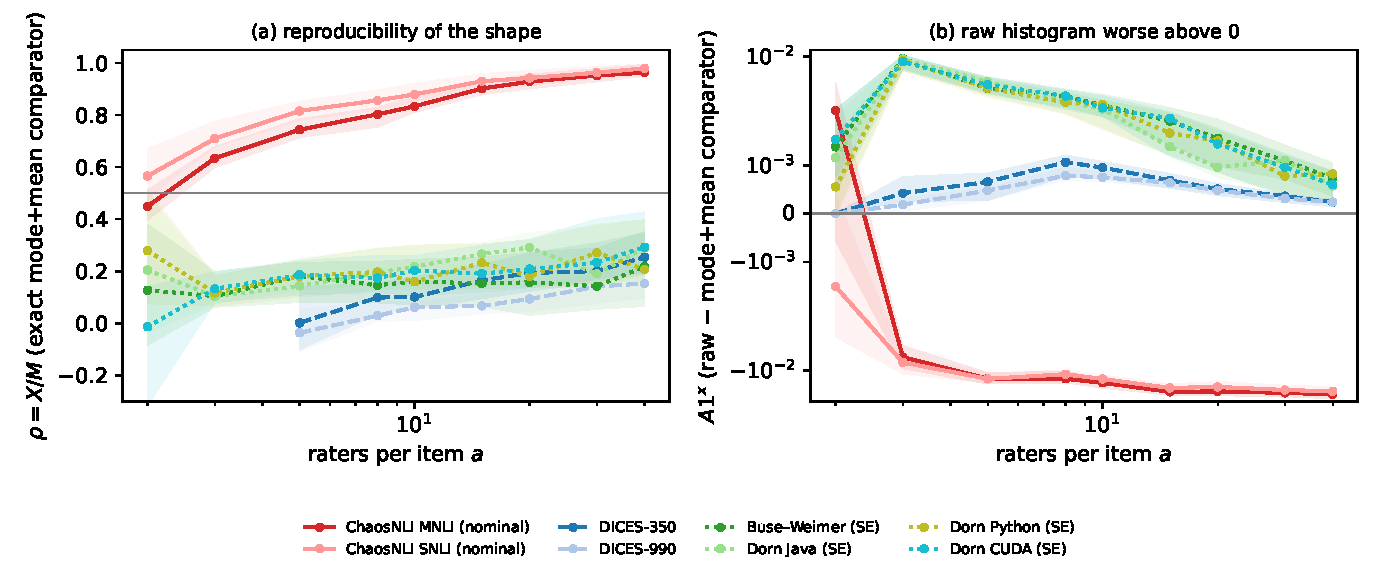
\includegraphics[width=\linewidth]{fig_reliability.pdf}\caption{Reliability of the shape beyond exact mode and mean against the number of raters per item, dense panels. (a) Split-half reliability $\rho=X/M$ relative to the exact mode-and-mean comparator, with 95\% item-cluster intervals; omitted where the residual is structurally empty or the ratio interval is wider than 1 (DICES with 2--5 ratings on a 3-level scale). The raw histogram beats the location-only forecast only above $\tfrac12$. (b) $A1^x$: positive means the raw histogram forecasts a new rater worse than its own mode and mean.}\label{fig:reliability}\end{figure}


\textbf{Setting.} Item \(i\) has ratings on \(K\) ordered levels, with empirical histogram \(h_i\). We score ordinal forecasts with the ranked probability score \(S(f,y)=\sum_k (F_f(k)-\mathbf 1[y\le k])^2/(K-1)\) and write \(C\) for the cumulative operator. For nominal tasks (ChaosNLI), \(S\) is the Brier score and \(C\) is the identity.

The \emph{location} of a histogram is its exact mode and mean; for nominal tasks it is the modal class and modal mass. To isolate the \emph{shape beyond location} we use the exact-T comparator \(q_T\): a cross-fitted forecast built from other items in the same exact mode-and-mean cell. It is KL-projected onto the cell when the cell is sparse (Appendix A). By construction \(q_T\) has the same location as \(h_i\) and differs from it only in shape. The residual of a histogram is \(r = C(h - q_T)\).

\textbf{Split-half identity.} In each repetition, every item's ratings are split at random into disjoint panels \(P_1\) (size \(a\)) and \(P_2\). Let \(r_1 = C(h_1-q_T)\) and \(r_2 = C(h_2-q_T)\), with \(q_T\) computed from \(P_1\). The value of the raw histogram over the comparator for forecasting a rating in \(P_2\) then obeys the exact identity \[A1 = \mathbb E\big[S(h_1,y)-S(q_T,y)\big]_{y\in P_2} = M - 2X,\] with \(M=\|r_1\|^2/n\) and \(X=\langle r_1,r_2\rangle/n\). Here \(\langle u,v\rangle=\sum_k u_k v_k/(K-1)\). Hence \(\rho = X/M\) is a \emph{new-rater forecasting reliability}: the raw histogram beats the location-only forecast exactly when \(\rho>\tfrac12\).

\textbf{Own versus cross reproducibility.} Because \(r_2\) is measured against panel 1's comparator, \(X\) is not purely agreement between the two panels' shapes. Writing \(q_j\) for the comparator built from panel \(j\), it splits as \(X = X_{\rm own} + X_{\rm cross}\):

\begin{itemize}
\tightlist
\item
  \(X_{\rm own}=\langle r_1, C(h_2-q_2)\rangle/n\) is the agreement of the two shapes, each measured beyond its own location;
\item
  \(X_{\rm cross}=\langle r_1, C(q_2-q_1)\rangle/n\) is panel 1's residual predicting the other panel's location shift.
\end{itemize}

The cross-term is not negligible. It is 31--40 \% of \(X\) on ChaosNLI at \(a=20\), and about half or more of \(X\) on the ordinal dense panels at \(a\le 8\). We therefore treat \(\rho\) as a forecasting quantity and use \(\rho_{\rm own}=X_{\rm own}/M\) for the reproducibility of the shape itself.

\textbf{Intervals and population.} Intervals are item-cluster bootstraps that refit the comparator in every replicate. Where raters recur across items, these intervals condition on the observed rater pool. For the three complete crossed panels we add crossed item $\times$ rater bootstraps. Where rating columns are anonymous positions, the intervals refer to new raters only if the positions are filled independently across items (Appendix A).

\textbf{Results.} Table~\ref{tab:cards} gives the resulting \emph{reliability cards}, and Figure~\ref{fig:reliability} traces \(\rho\) against \(a\) on the dense panels.

\emph{Ordinal panels.}

\begin{itemize}
\tightlist
\item
  With 4--8 raters per item, $\rho$ is 0.04--0.41 on eight panels, and the intervals include 0 on four.
\item
  On SummEval's non-duplicated items it falls to 0.10 and 0.05, with intervals including 0 (Appendix C).
\item
  With three raters, $\rho$ cannot be measured. A split leaves two ratings per item, and two ratings are determined by their exact mode and mean under our tie rule, although 15--75 \% of the three-rating histograms share their exact cell with a different histogram.
\item
  On the dense ordinal panels $\rho$ stays below 0.3 up to 40 raters: Buse--Weimer 0.22, DICES 0.25 and 0.15, and Dorn's Java panel 0.29.
\item
  Under crossed item $\times$ rater bootstraps the $\rho$ upper bounds stay below $\tfrac12$ (BW 0.39, DICES-350 0.36 at 40 raters, rounded outward).
\end{itemize}

\emph{NLI.} On ChaosNLI, $\rho$ exceeds $\tfrac12$ from two to three raters and reaches 0.96--0.98 at 40.

\emph{The shape itself.} At 40 raters, $\rho$\_own is 0.06--0.22 on the dense ordinal panels: BW 0.13, DICES-350 0.10, DICES-990 0.06, Dorn 0.12--0.22. With rater resampling the BW and DICES-350 intervals include 0, with upper bounds $\leq$ 0.26. On MNLI / SNLI, $\rho$\_own is 0.61 / 0.67.

For new raters, then, we bound the ordinal shape-to-shape reproducibility from above rather than show it to be positive. The ordinal--NLI contrast holds on both measures.

\section{Reliability across text}
\begin{table*}[t]\centering\footnotesize
\caption{Own-shape decoding: the cross-fitted decoder's gain against panel 2's residual from its own mode and mean, as a percentage of the reproducible own-shape, $100\,G_{\rm own}/X_{\rm own}$, and net of the within-cell permutation (decoder variance penalty); $X_{\rm own}$ in units of $10^{-4}$. Item-cluster CLT 95\% intervals (\S4). $a/b$: raters in panel 1 / panel 2. No ratio where $X_{\rm own}$'s interval covers 0. SummEval full-panel rows include the duplicated crowd annotations; non-dup.\ rows exclude them (Appendix~C). HelpSteer2 and EmoBank ($b=2$) cannot measure the own-shape.}\label{tab:own}
\begin{tabular}{lrllll}\toprule panel & $a/b$ & features & $X_{\rm own}$ & $G_{\rm own}/X_{\rm own}$ (\%) & net (\%) \\\midrule
DICES-350 & 20/20 & Qwen2.5 & $+$0.44 [$+$0.05, $+$0.83] & $-$8.0 [$-$23.0, $+$7.1] & $+$11.6 [$-$6.2, $+$29.4] \\
DICES-350 & 20/20 & OLMo-2 & $+$0.44 [$+$0.05, $+$0.83] & $-$4.7 [$-$13.2, $+$3.7] & $+$8.9 [$-$2.7, $+$20.5] \\
DICES-350 & 20/20 & Qwen3 & $+$0.44 [$+$0.05, $+$0.83] & $-$0.4 [$-$7.5, $+$6.8] & $+$8.8 [$-$1.9, $+$19.4] \\
DICES-350 & 40/20 & Qwen2.5 & $+$0.49 [$+$0.16, $+$0.82] & $+$1.3 [$-$8.8, $+$11.4] & $+$15.0 [$+$2.6, $+$27.4] \\
DICES-350 & 40/20 & OLMo-2 & $+$0.49 [$+$0.16, $+$0.82] & $-$0.0 [$-$7.2, $+$7.2] & $+$6.8 [$-$1.9, $+$15.6] \\
DICES-350 & 40/20 & Qwen3 & $+$0.49 [$+$0.16, $+$0.82] & $-$0.6 [$-$8.0, $+$6.8] & $+$9.5 [$-$0.3, $+$19.3] \\
DICES-990 & 20/20 & Qwen2.5 & $+$0.22 [$-$0.02, $+$0.45] & $X_{\rm own}$ n.s. & -- \\
Dorn (all)$^{SE}$ & 20/20 & Qwen2.5 & $+$2.73 [$+$2.03, $+$3.43] & $+$10.2 [$+$4.4, $+$15.9] & $+$11.4 [$+$7.1, $+$15.8] \\
Dorn Java$^{SE}$ & 20/20 & Qwen2.5 & $+$2.69 [$+$1.55, $+$3.84] & $+$0.3 [$-$14.9, $+$15.5] & $+$11.3 [$+$2.7, $+$19.9] \\
EmoBank & 3/2 & Qwen2.5 & $+$0.02 [$-$0.02, $+$0.06] & $X_{\rm own}$ n.s. & -- \\
HelpSteer2 & 3/2 & Qwen2.5 & $+$0.00 [$+$0.00, $+$0.00] & $X_{\rm own}$ n.s. & -- \\
POPQUORN off. & 4/4 & Qwen2.5 & $-$0.08 [$-$1.14, $+$0.99] & $X_{\rm own}$ n.s. & -- \\
SummEval coh.\ (full panel) & 4/4 & Qwen2.5 & $+$3.75 [$+$2.45, $+$5.05] & $+$0.9 [$-$0.3, $+$2.0] & $+$2.2 [$+$1.0, $+$3.4] \\
SummEval coh.\ (full panel) & 4/4 & OLMo-2 & $+$3.75 [$+$2.45, $+$5.05] & $+$0.7 [$-$0.4, $+$1.8] & $+$3.1 [$+$1.5, $+$4.7] \\
SummEval coh.\ (full panel) & 4/4 & Qwen3 & $+$3.75 [$+$2.45, $+$5.05] & $+$1.7 [$+$0.6, $+$2.8] & $+$3.1 [$+$1.6, $+$4.6] \\
SummEval coh.\ (non-dup.) & 4/4 & Qwen2.5 & $-$1.33 [$-$2.98, $+$0.31] & $X_{\rm own}$ n.s. & -- \\
SummEval rel.\ (full panel) & 4/4 & Qwen2.5 & $+$3.07 [$+$1.83, $+$4.31] & $+$1.3 [$+$0.1, $+$2.5] & $+$2.9 [$+$1.4, $+$4.4] \\
SummEval rel.\ (non-dup.) & 4/4 & Qwen2.5 & $-$0.32 [$-$1.64, $+$1.00] & $X_{\rm own}$ n.s. & -- \\
ChaosNLI MNLI & 4/4 & Qwen2.5 & $+$41.62 [$+$36.40, $+$46.84] & $+$22.0 [$+$18.7, $+$25.4] & $+$30.7 [$+$26.8, $+$34.7] \\
ChaosNLI MNLI & 20/20 & Qwen2.5 & $+$111.31 [$+$102.32, $+$120.31] & $+$28.3 [$+$24.6, $+$32.0] & $+$36.5 [$+$32.8, $+$40.2] \\
ChaosNLI MNLI & 20/20 & OLMo-2 & $+$111.31 [$+$102.32, $+$120.31] & $+$28.9 [$+$25.4, $+$32.4] & $+$36.4 [$+$32.9, $+$39.9] \\
ChaosNLI MNLI & 20/20 & Qwen3 & $+$111.31 [$+$102.32, $+$120.31] & $+$30.2 [$+$26.7, $+$33.8] & $+$38.2 [$+$34.7, $+$41.8] \\
ChaosNLI SNLI & 4/4 & Qwen2.5 & $+$35.23 [$+$30.41, $+$40.05] & $+$28.4 [$+$24.8, $+$31.9] & $+$36.4 [$+$32.1, $+$40.6] \\
ChaosNLI SNLI & 20/20 & Qwen2.5 & $+$111.94 [$+$102.04, $+$121.84] & $+$37.8 [$+$34.0, $+$41.6] & $+$45.2 [$+$41.2, $+$49.1] \\
\bottomrule\end{tabular}\end{table*}

\textbf{Decoder.} A judge sees the text, not the raters. We ask whether the reproducible shape is available in the representation the judges are built on: last-token hidden states of frozen Qwen2.5-7B-Instruct (Qwen2.5-Coder for code panels) under the rating prompt. Qwen3-8B and OLMo-2-7B serve as second and third families.

A multi-output ridge decoder predicts \(r_1\) from the features. It is group-cross-fitted over five item folds, with a label-free PCA and a nested penalty. We score it on panel 2's residual measured from its own exact cell, \(s_2 = C(h_2-q_2)\), by the proper-score gain \[G_{\rm own} = \big(2\langle\hat r,s_2\rangle-\|\hat r\|^2\big)/n .\] This gain measures the shape alone. It excludes the part of the full gain that comes from predicting panel 2's location shift; the full, cross-term-inclusive ratio \(G/X\) is reported in Appendix B. The headline estimand is \(G_{\rm own}/X_{\rm own}\), reported where \(X_{\rm own}\)'s interval excludes 0.

Intervals are item-cluster CLT intervals on per-item contributions, averaged over ten cross-fitting repetitions with the predictions held fixed. Ratios get delta-method intervals. As a check fixed in advance, the interval for \(\langle\hat r,s_2\rangle/n\) covers 0 in 9 of 10 null draws (Appendix A).

\textbf{Controls.} Every estimate has three controls:

\begin{enumerate}
\def\labelenumi{\arabic{enumi}.}
\tightlist
\item
  A \emph{within-cell permutation} of the features among items with the same exact mode and mean. Under this control \(G_{\rm own}\) must be at or below zero; its null expectation is \(-E\|\hat r\|^2/n\), the decoder's variance penalty.
\item
  A \emph{positive control} that predicts the panel-1 mean with the same pipeline.
\item
  A \emph{planted shape} used to calibrate power. Item dispersion is made log-linear in a random feature direction, with $\gamma$ setting the strength, and is simulated with the panel's fitted rater cut-points. We call the plant detected when the CLT lower bound of \(G_{\rm own}\) exceeds 0. For Dorn and DICES-350, the reference strength is the smallest $\gamma$ whose mean planted \(X_{\rm own}\) reaches the observed one; the rule prespecified for SummEval and POPQUORN compares \(X\) instead (Appendix B).
\end{enumerate}

\textbf{Pool bias.} Within the observed rater pool, \(X_{\rm own}\) is biased downward for new raters. This happens because each item's halves are drawn without replacement from one pool of raters with different cut-points, so the rater mixes of the two halves are anti-correlated. Simulations from the fitted rater--item model locate this bias (Appendix A). It makes ``no detectable own-shape'' easier to declare, and we read the nulls below accordingly.

\textbf{Results (Table~\ref{tab:own}).}

\emph{Where an own-shape is detectable at all.} The ordinal own-shape is undetectable on SummEval's non-duplicated items, POPQUORN (\(a=4\)) and DICES-990 (\(a=20\)); on these panels \(G_{\rm own}\) $\approx$ 0. Two ordinal panels have a detectable own-shape:

\begin{itemize}
\tightlist
\item
  On Dorn's readability panel the decoder recovers 10 \% {[}4, 16{]}. However, a pure location-and-threshold simulation of Dorn's Java panel already yields a text-decodable own-shape: over five draws its \(\langle\hat r, s_2\rangle\) averages about 95 \% of the value observed on the real panel. A plant matching the observed magnitude is detected in only 1 of 5 draws. Dorn's 10 \% is therefore an upper bound, of the size location alone produces.
\item
  On DICES-350 the decoder recovers $-$8 \% {[}$-$23, 8{]} at 20 raters per half and 1 \% {[}$-$9, 12{]} at 40.
\end{itemize}

\emph{NLI.} The decoder recovers 28 \% {[}24, 33{]} on MNLI and 38 \% {[}33, 42{]} on SNLI. With four raters per half, ChaosNLI still gives 22 \% {[}18, 26{]} and 28 \% {[}24, 32{]}.

\emph{The NLI--ordinal gap.} Every NLI lower bound exceeds every ordinal upper bound: 24 \% vs 16 \% at 20 raters per half, 18 \% vs 3 \% at 4. The gap also holds net of the variance penalty, \((G_{\rm own}-G_{\rm own,perm})/X_{\rm own}\), at 20 raters per half: at most 30 \% on the ordinal panels against at least 32 \% on NLI.

\emph{DICES-350 at 40 raters, the clean ordinal case.}

\begin{itemize}
\tightlist
\item
  A location-and-threshold simulation of the panel yields no own-shape at all: mean \(X_{\rm own}\) is $-$1.3$\cdot$10$^{-}$$^{5}$, against the observed 4.9$\cdot$10$^{-}$$^{5}$. A reproducible ordinal shape beyond location therefore exists here within the observed rater pool.
\item
  A planted text-predictable dispersion shape of matching magnitude is detected in 5 of 5 draws and recovered at 15--33 \%. A polarisation plant of matching magnitude is detected in only 3 of 5 (\S{}7).
\item
  Against this, the observed recovery is $-$1 to 1 \% across the three feature families, with upper bounds $\leq$ 12 \%.
\item
  The decoder's covariance with the other half's shape, \(V_{\rm own}=\langle\hat r,s_2\rangle/n\), is nonetheless positive in all three families (4.9, 2.8 and 2.3$\cdot$10$^{-}$$^{6}$, about ten times the simulation's 4.7$\cdot$10$^{-}$$^{7}$); the variance penalty cancels it (net of the penalty, 15 \% {[}3, 27{]} on Qwen2.5).
\end{itemize}

On DICES-350, then, the shape exists within the observed rater pool, the decoder has power for a planted shape of this size and construction, and the observed shape tracks the text only weakly: detectably, but with no proper-score gain (ROUND23 R23-1, a post-hoc reporting change).

\emph{Robustness.} Qwen3-8B and OLMo-2-7B give the same readings (MNLI 30 \% and 29 \%); own-shape decoding on all three families covers SummEval, MNLI and DICES-350, the other panels are Qwen2.5 only. A nonlinear random-feature decoder (SummEval and POPQUORN only), the cross-term-inclusive ratio \(G/X\), and a valid-forecast version projected onto the exact cell all agree (Appendices A--B). Scored as a valid forecast, the permutation-corrected gain is $\leq$ 6$\cdot$10$^{-}$$^{5}$ RPS on the ordinal panels, against 0.0065 and 0.0072 on MNLI and SNLI.

\textbf{Why the two reliabilities can come apart.} \(\rho\) asks whether the shape is a property of an item's rater population, and \(G_{\rm own}\) asks whether it is a property of the item's text. A shape can be reproducible yet invisible to text, for instance when it arises from how particular raters use the scale. Section 5 shows that, on the panels with persistent rater identities, most held-out likelihood structure beyond item location is associated with who rated.

\section{What learned judges use}

\textbf{Donor-replacement audit.} If a judge learned the shape beyond location, destroying that shape in its training targets would hurt it. The audit replaces the histogram of 69--83 \% of training items by another item's histogram, projected onto the recipient's exact mode and mean. Among changed items the mean total-variation distance is 0.30--0.35. We run it under two learners (Appendix D gives the full design).

\emph{LoRA judges.} These are end-to-end judges on Qwen2.5-7B-Instruct with the distributional objective of \citet{chen2025beyond}, trained with three optimizer--assignment realisations $\times$ three held-out-rater folds.

\begin{itemize}
\tightlist
\item
  Shape replacement changes held-out RPS by $-$0.0001 {[}$-$0.0011, +0.0011{]} on SummEval coherence and +0.0000 {[}$-$0.0009, +0.0009{]} on POPQUORN offensiveness.
\item
  Destroying the location as well (mode-only replacement) costs +0.0120 {[}+0.0086, +0.0155{]} and +0.0029 {[}+0.0009, +0.0050{]}, with every seed-by-fold cell positive.
\item
  On POPQUORN, resampling users instead of rating positions widens these intervals to {[}$-$0.0014, +0.0015{]} and {[}$-$0.0004, +0.0065{]}.
\end{itemize}

\emph{Frozen-feature heads.} On ten ordinal panels, heads move by $-$0.0024 to +0.0006.

\textbf{ChaosNLI, the discriminating case.} On SummEval's non-duplicated items and on POPQUORN no own-shape is detectable (\S{}4), so a null there is the expected outcome rather than independent evidence. On the nominal ChaosNLI panels, the shape is both reproducible and decodable. There, the same kind of intervention scrambles the allocation of mass beyond the modal class while preserving the modal mass. It raises the test Brier score at every annotation count:

\begin{itemize}
\tightlist
\item
  by 0.005--0.012 on MNLI and 0.008--0.017 on SNLI (KL 0.016--0.052);
\item
  equivalently, by 0.29--1.31 of the Brier gap between an oracle that uses the item's own training histogram and the exact comparator.
\end{itemize}

On binary $\alpha$NLI, where the replacement cannot change any target, the same contrast is a sham and averages $-$0.003 to +0.002.

\textbf{Any target construction.} We also trained heads on eleven ordinal panels with each of the following target constructions, thirty configurations each:

\begin{itemize}
\tightlist
\item
  the raw histogram;
\item
  the location-only comparator;
\item
  reliability-shrunk shapes and locations;
\item
  Dirichlet and label smoothing;
\item
  a cross-item smoothed comparator;
\item
  one-hot labels.
\end{itemize}

The results:

\begin{itemize}
\tightlist
\item
  The location-only comparator and the reliability-shrunk shapes change held-out RPS by at most 0.0012, with mixed signs.
\item
  The other smoothing constructions move it by $-$0.005 to +0.009, in directions that differ across panels.
\item
  One-hot targets are worse on 10 of 11 panels.
\end{itemize}

The learner pools location across items on its own and shows no sensitivity to the per-item shape. That is what \S{}4 predicts for a shape that is not decodable from its features.

\textbf{Where the ordinal structure beyond location lives.} We fit ordered-probit models \(Y^*_{ir} = \theta_i + \sigma_i\varepsilon_{ir}\) with cut-points \(c_r\) to the panels with persistent rater identities, and location-plus-dispersion models to the position panels:

\begin{itemize}
\tightlist
\item
  M0 has item location and common cut-points;
\item
  M1 adds rater-specific cut-points;
\item
  M2 adds item-specific dispersion.
\end{itemize}

Rater thresholds carry the structure. M1 improves held-out likelihood by 0.05--0.16 nats per rating, whereas item dispersion adds $-$0.017 to +0.012.

Simulating from the fitted models and re-running the split-half analysis at 40 + 20 raters does not single out a model:

\begin{itemize}
\tightlist
\item
  On DICES-350, no model reproduces the observed \(X_{\rm own}\); the threshold model generates none.
\item
  On Buse--Weimer, only the dispersion model does.
\item
  On Dorn's Java panel, the observed value lies between the location-only and dispersion ranges.
\end{itemize}

An earlier run with fewer split repetitions read differently on every panel (Appendix F), so we draw no conclusion from this comparison.

At smaller splits, the location-only model reproduces most of the observed \(X\) through \(X_{\rm cross}\) (Appendix F). This is the textbook mechanism of many-facet Rasch measurement (\citealp{linacre1989mfrm}; \citealp{eckes2011mfrm}), which we present as measurement, not as a claim about raters' psychology. On the panels with persistent rater identities, most of the held-out likelihood structure beyond item location is associated with who rated, and a judge that sees only the text cannot learn that part. Whether the residual shape itself is rater-side is not established on any panel.

\section{Annotation budget}
\begin{table}[t]\centering\footnotesize
\caption{End-to-end LoRA judges on POPQUORN offensiveness at fixed rating budgets, prospective block with independent rating assignments (Qwen2.5-7B, R20-4): test RPS minus the full-data judge, 95\% crossed bootstrap over optimizer seeds and test groups. All blocks, including SummEval (expert dilution), are in Table~\ref{tab:budget}.}\label{tab:budgetmain}
\resizebox{\columnwidth}{!}{\begin{tabular}{llrrl}\toprule panel & design (items $\times$ ratings) & ratings & RPS & $-$ full data \\\midrule
POPQUORN & 819 $\times$ 1 & 819 & 0.1278 & $+$0.0063 [$+$0.0030, $+$0.0099] \\
POPQUORN & 117 $\times$ 7 & 819 & 0.1305 & $+$0.0090 [$+$0.0056, $+$0.0124] \\
POPQUORN & 819 $\times$ 2 & 1638 & 0.1247 & $+$0.0032 [$+$0.0016, $+$0.0048] \\
POPQUORN & 819 $\times$ 7 & 5733 & 0.1215 & -- \\
\bottomrule\end{tabular}}\end{table}


We test the budget question directly, as an observation in its own right: hold the total number of ratings fixed and trade items for raters. We do not derive the answer from \S{}\S{}3--5. A registered mechanism-based prediction failed on ChaosNLI (\S{}1).

\textbf{Frozen-feature heads} (eight ordinal and two nominal panels, thirty configurations each; Appendix F). On four of the five panels with more than 900 training items, more items with fewer ratings each wins monotonically. On DICES-990 at a budget of 594 ratings, for example, RPS rises steadily as ratings are concentrated on fewer items: 594 items $\times$ 1 rating gives 0.203, 297 $\times$ 2 gives 0.205, 148 $\times$ 4 gives 0.207, 74 $\times$ 8 gives 0.213 and 40 $\times$ 15 gives 0.219.

SummEval is flat. The direction reverses only on small item sets (60 and 210 training items), where a single rating per item is too noisy a target. The items-first order also holds on ChaosNLI (959 $\times$ 1: KL 0.226; 30 $\times$ 32: 0.323). What differs between tasks is the \emph{marginal} value of a second rating on items already covered: $-$12 to $-$15 \% on ChaosNLI against $-$1 to $-$3 \% for the Qwen2.5 heads on the large ordinal panels.

\textbf{LoRA judges on POPQUORN} (Table~\ref{tab:budgetmain}). POPQUORN offensiveness has homogeneous rating positions, which makes it the clean budget case. Every arm trains for the same number of optimizer steps, and all contrasts are taken within one batch, because LoRA training on our hardware is not bit-reproducible: per-cell RPS varies by $\leq$ 0.0012 between identical runs. A prospective block with independent rating assignments (ROUND20 R20-4) gives:

\begin{itemize}
\tightlist
\item
  819 $\times$ 1 $-$ full = +0.0063 {[}+0.0030, +0.0099{]}: one rating per item is worse than the full data.
\item
  819 $\times$ 2 $-$ 819 $\times$ 1 = $-$0.0031 {[}$-$0.0062, $-$0.0002{]}: a second rating recovers 49 \% of that gap.
\item
  117 $\times$ 7 $-$ 819 $\times$ 1 = +0.0027 {[}$-$0.0024, +0.0074{]}: items-first is not supported.
\end{itemize}

The earlier same-batch block gives the same three readings, with 819 $\times$ 1 $-$ full = +0.0087 {[}+0.0054, +0.0122{]} and 62 \% recovered by a second rating.

\textbf{SummEval measures dilution, not budget.} The evaluator is a held-out expert and the crowd mean barely tracks the expert mean (r = 0.04), so ``fewer ratings per item'' changes how far the expert ratings are diluted; those blocks are in Appendix C.

\textbf{Guidance, conditional on task and learner.}

\begin{itemize}
\tightlist
\item
  For ordinal rating tasks with more than 900 items, frozen-feature heads favour covering items first (SummEval is flat; HelpSteer2 on OLMo-2 is the exception); on $\leq$ 210 training items the direction reverses.
\item
  With LoRA judges (POPQUORN), two ratings per item are a safer default than one.
\item
  Where the rater pool mixes populations, who rates matters more than how many ratings are collected.
\item
  Many raters per item belong where a reliable reference distribution is itself the deliverable: evaluation sets, and tasks such as NLI where the shape is in the text.
\end{itemize}

\section{Limitations and conclusion}

\textbf{Limitations.}

\begin{itemize}
\tightlist
\item
  \emph{Learners and decoders.} The frozen-feature analyses use three model families, but own-shape decoding on all three covers only SummEval, MNLI and DICES-350; the other panels and the valid-forecast gain are Qwen2.5 only. The SummEval LoRA contrasts (Appendix C) replicate on OLMo-2-7B; the POPQUORN budget block and the LoRA audit are Qwen2.5 only. We test linear decoders and one non-linear probe (on SummEval and POPQUORN only), not fine-tuned probes.
\item
  \emph{Plant scope.} The main plant is one construction: item log-dispersion linear in one feature direction. At \(a=20\) (Dorn) the matched plant is detected in 1 of 5 draws, at \(a=40\) (DICES-350) in 5 of 5, and there are no plants on NLI. A second construction on DICES-350, text-predictable polarisation of two fixed rater groups (ROUND22 R22-6, grid amended after a smoke run), reaches the observed own-shape magnitude at $\gamma$ = 1.5. There it is detected in only 3 of 5 draws, with recovery of 1--22 \%, so the DICES-350 null is informative against the dispersion construction but not against polarisation.
\item
  \emph{Exact cells and the rater pool.} At 20 raters the exact (mode, mean) cell pools items of different latent location, so a decodable own-shape can be location-driven. The ordinal fractions are therefore upper bounds on shape beyond location, and the NLI values may contain such a component. The pool bias of \S{}4 makes ``no detectable own-shape'' slightly easier to declare.
\item
  \emph{SummEval data.} The released file has identical crowd annotations on 807 of 1,600 items. This is undocumented and unverified upstream. It makes SummEval's full-panel numbers artefactual and its budget contrasts dilution contrasts (Appendix C).
\item
  \emph{POPQUORN position folds.} A user-held-out check with real user ids, in which no evaluator contributes to any target, confirms the audit and budget conclusions.
\item
  \emph{Effect sizes.} The effects lie in the third decimal of RPS. They should be read against the mode-only penalty of +0.012 and the POPQUORN budget effects of 0.006--0.009.
\end{itemize}

\textbf{Conclusion.} A few-rater histogram is a noisy location plus a shape that, on ordinal scales, is barely reproducible across raters and, where it is reproducible, gives no proper-score gain when decoded linearly from the frozen features we tested. On DICES-350 the shape exists within the rater pool and a planted shape of its size is decoded; the real one covaries with the text only weakly.

On NLI the shape is reproducible and a quarter to two-fifths of it is decodable. Learned judges follow the same split. For the budget, frozen-feature heads on ordinal panels with more than 900 items favoured covering items first, while for LoRA judges on POPQUORN two ratings per item beat one, an observation rather than a consequence of the mechanism. Reliability cards allow that check before rating starts.

\bibliographystyle{plainnat}
\bibliography{../references}
\onecolumn
\appendix

Sections A--F give the full estimator definitions and the complete results behind the main text. Their text follows the long version of the paper (PAPER\_DRAFT\_v2.md, v2.5); the main text quotes their numbers verbatim.

\section{Estimators}

\textbf{Setting and notation.} Item \(i\) has ratings on \(K\) ordered levels from a panel of raters; the empirical histogram is \(h_i\). For ordinal scales we score forecasts with the ranked probability score, \(S(f,y)=\sum_k (F_f(k)-\mathbf 1[y\le k])^2/(K-1)\), and write \(C\) for the cumulative operator; for nominal tasks (ChaosNLI) \(S\) is the Brier score and \(C\) the identity. The \textbf{location} of a histogram is its exact mode and mean (nominal: modal class and modal mass); the \textbf{shape beyond location} is what remains once these are fixed. To isolate it we use the \emph{exact-T comparator} \(q_T\): a cross-fitted forecast built from other items in the same exact mode-and-mean cell (KL-projected onto the cell when the cell is sparse), so that \(q_T\) has the same mode and mean as \(h_i\) and differs from it only in shape. The residual of a histogram is \(r = C(h - q_T)\).

\textbf{A.1 Reproducibility across raters (split-half reliability).} In each of \(R\) repetitions the ratings of every item are split at random into disjoint panels \(P_1\) (size \(a\)) and \(P_2\). Writing \(r_1 = C(h_1-q_T)\) and \(r_2 = C(h_2-q_T)\), with \(q_T\) computed from \(P_1\), the forecasting value of the raw histogram over the comparator obeys the exact identity \[A1 \;=\; \mathbb E\big[S(h_1,y)-S(q_T,y)\big]_{y\in P_2} \;=\; M - 2X,\qquad M=\|r_1\|^2/n,\; X=\langle r_1,r_2\rangle/n,\] where \(\langle u,v\rangle=\sum_k u_k v_k/(K-1)\) for ordinal scales (the RPS normalisation; 1 for nominal), so the identity is exact as implemented. Thus \(\rho = X/M\) is a \textbf{new-rater forecasting reliability}: the raw histogram beats the location-only forecast exactly when \(\rho>\tfrac12\). Because \(r_2\) is taken against panel 1's comparator, \(X\) is not purely shape-to-shape agreement: writing \(q_j\) for the comparator built from panel \(j\), \(X = X_{\text{own}} + X_{\text{cross}}\) with \(X_{\text{own}}=\langle r_1, C(h_2-q_2)\rangle/n\) (agreement of the two panels' shapes, each beyond its own location) and \(X_{\text{cross}}=\langle r_1, C(q_2-q_1)\rangle/n\) (panel 1's residual predicting the other panel's location shift). On the dense panels we report both; the cross-term is not negligible (31--40 \% of \(X\) on ChaosNLI at \(a=20\); about half or more of \(X\) on the ordinal dense panels at \(a\le 8\)), so we call \(\rho\) a forecasting quantity and use \(\rho_{\text{own}}=X_{\text{own}}/M\) for the reproducibility of the shape itself. On the small panels the second panel is a single rating, its own comparator is that rating, and \(X_{\text{own}}\equiv 0\): there \(\rho\) is by construction a statement about forecasting a new rater. \(\rho\) is specific to the number of raters \(a\) and, as a ratio, unstable when \(M\) is tiny; we report it with intervals and omit it where the residual is structurally empty (e.g.~two or three ratings on a three-level scale). We also report the support of the donor-replacement intervention (the fraction of items whose histogram could be changed at all while preserving mode and mean). A smoother, response-based comparator that does not reproduce the noisy location gives larger values of \(\rho\) because it also credits location reliability; we use the exact comparator throughout. Intervals are item-cluster bootstraps in which all copies of a resampled item stay in one cross-fitting fold and the comparator is refitted in every replicate. \emph{Population.} On panels whose rating columns are positions rather than persistent people (HelpSteer2, EmoBank, CSC, ChaosNLI, Dorn and the SE panels without identities), the item bootstrap resamples an item's ratings with the item, so the intervals refer to new raters \emph{if} the anonymous positions are filled by different people independently across items --- an assumption the datasets do not document. SummEval is mixed: its three expert columns are persistent people (intervals condition on them), its five crowd columns are positions; the crowd mean is nearly uncorrelated with the expert mean (r = 0.04; Fabbri et al., 2021), and on half of the released items the five crowd annotations are identical on all four dimensions, an undocumented pattern we could not verify upstream (Appendix C, ROUND22). Where raters recur across items (Buse--Weimer, DICES-350, DICES-990, Scalabrino, POPQUORN), item-cluster intervals condition on the observed rater pool; for the three complete crossed panels we also report crossed item $\times$ rater bootstrap intervals: the $\rho$ upper bounds stay below the $\tfrac12$ forecasting threshold (BW 0.39, DICES-350 0.36 at 40 raters; DICES-990 0.10 at 10 raters, the largest feasible; rounded outward) --- this supports ``below $\tfrac12$'' for new raters, not the ``below 0.3'' of the point estimates, but $\rho$\_own's intervals then include 0 on BW and DICES-350 ({[}$-$0.004, 0.26{]}, {[}$-$0.02, 0.19{]}), so for new raters we bound the ordinal shape-to-shape reproducibility above rather than show it positive, and for POPQUORN the LoRA comparisons are additionally given under user-level clustering (Appendix D). Table~\ref{tab:cards} gives the resulting \emph{reliability cards}; Figure~\ref{fig:reliability} traces \(\rho\) and \(A1^x = M-2X\) (the score change of the raw histogram over the exact comparator when forecasting a held-out rating; negative means the raw histogram is better) against \(a\) on the dense panels.

\textbf{A.2 Predictability from the text (decodability).} A judge sees the text, not the raters. Whether the reproducible shape is available to it is a separate question, which we answer with the representation the judges are built on: last-token hidden states of the frozen Qwen2.5-7B-Instruct (Qwen2.5-Coder for code panels) under the same rating prompt. A multi-output ridge decoder, group-cross-fitted over five item folds with a label-free PCA and a nested penalty, predicts \(r_1\) from the features; it is scored on the \emph{independent} panel \(r_2\) by the covariance \(V=\langle\hat r,r_2\rangle/n\) and by the proper-score gain \[G \;=\; \big(2\langle \hat r, r_2\rangle - \|\hat r\|^2\big)/n \;=\; \mathbb E_{y\in P_2}\big[S(q_T,y) - S(q_T + C^{-1}\hat r,\,y)\big],\] the exact reduction in score obtained by adding the decoded shape to the location-only forecast. Two controls accompany every estimate: a \emph{within-cell permutation} of the features among items with the same exact mode and mean (which must drive \(G\) to zero or below), and a \emph{positive control} that predicts the panel-1 mean with the same pipeline (which must be clearly positive, else the representation or the alignment is broken). A third control calibrates power: we plant a known, text-predictable shape (item dispersion log-linear in a random direction of the features, with the panel's fitted locations and cut-points) and rerun the unchanged pipeline. \textbf{Own-shape decomposition (ROUND20 R20-1).} With \(s_2=C(h_2-q_2)\) (panel 2's residual from its own exact cell) and \(d=C(q_2-q_1)\), the gain splits as \(G=G_{\rm own}+G_{\rm cross}\), with \(G_{\rm own}=(2\langle\hat r,s_2\rangle-\|\hat r\|^2)/n\) and \(G_{\rm cross}=2\langle\hat r,d\rangle/n\), and likewise \(X=X_{\rm own}+X_{\rm cross}\) (\S{}3). The headline estimand is \(G_{\rm own}/X_{\rm own}\), reported where \(X_{\rm own}\)'s interval excludes 0; we call \(G/X\) the \emph{normalised forecasting gain}. Reading the planted control on this scale: with no planted shape the permutation-corrected projected gain $\Delta$GP is zero on both panels in every draw. \(G_{\rm own}\) is slightly negative, as it must be: its expectation under the null is \(-E\|\hat r\|^2/n\), the decoder's variance penalty. Our frozen null check, which required its interval to cover 0, was therefore ill-posed; the uncorrected projected gain GP is positive under the null (the smoothing artefact described below). Over five simulation draws on SummEval (ROUND20 R20-2), the planted shape is detected (item-cluster CLT lower bound of G\_own \textgreater{} 0; ROUND22 R22-4) in 0 of 5 at $\gamma$ = 0, 5 of 5 at $\gamma$ = 0.3 and 5 of 5 at $\gamma$ = 0.6. At $\gamma$ = 0.6, \(X_{\rm own}\) is 0.00033--0.00047, bracketing SummEval's observed 0.00038, and the decoder recovers 38--56 \% of the planted own-shape (POPQUORN, five draws: detected in 5 of 5, 6--38 \%). The rule we fixed in advance compares the planted \(X\) with the observed \(X\). The first grid fell short (strongest plant 0.00166 against 0.00198), so we added $\gamma$ = 0.8 and 1.0 (ROUND20 R20-2a/c, written after seeing that). At $\gamma$ = 1.0 (mean planted X 0.00225) the plant is detected in 5 of 5 draws and recovered at 31--57 \%, so at its full-panel magnitude the SummEval null would be informative under the rule; but that magnitude is carried by the duplicated crowd annotations (ROUND22), so the calibration has no reproducible SummEval shape to refer to. On POPQUORN the reference plant ($\gamma$ = 0.3, X 0.00060 against the observed 0.00036) is detected in 2 of 5, so its null is uninformative. The planted own-shape saturates near 0.0004--0.0005 for $\gamma$ $\geq$ 0.6, close to SummEval's observed 0.00038; the 7--12 \% recovery under \(G/X\) (one R19-2 draw) came from the cross-term in the denominator. Two features of the estimator are post hoc and disclosed. First, at $\gamma$ = 0, \(X_{\rm own}\) is about $-$1$\cdot$10$^{-}$$^{4}$ although the halves are exchangeable (\(a=b=4\)). Simulations from the fitted rater--item model locate the cause (ROUND21 R21-2). Each item's two halves are drawn without replacement from one fixed pool of raters with different cut-points, so the halves' rater mixes are anti-correlated. With identical cut-points, or with raters drawn afresh for each rating, the bias vanishes (SummEval $-$0.000099 $\pm$ 0.000010 vs +0.000007 and +0.000018; DICES-350 $-$0.000015 $\pm$ 0.000003 vs $\approx$ 0; none on the panels fitted with one rater group). The real \(X_{\rm own}\) is therefore reproducibility within the observed rater pool, biased downward for new raters. That makes ``no detectable own-shape'' easier to declare: corrected for the pool effect, SummEval's full-panel \(X_{\rm own}\) is about 0.00048 (a correction from a rater model that cannot produce the duplicated crowd annotations, so it does not describe them), and DICES-350's interval at \(a=20\) only just covers 0. Second, the item bootstrap of \(G_{\rm own}\) duplicates items inside the cross-fit and is not centred on its point estimate. We therefore use item-cluster CLT intervals on the per-item contributions, averaged over ten cross-fitting repetitions with the cross-fitted predictions held fixed, so that no item is ever duplicated (ROUND21 R21-1). Ratios get delta-method intervals. As a check, fixed in advance, the interval for \(\langle\hat r,s_2\rangle/n\), which has mean 0 under the no-plant null, covers 0 in 9 of 10 null draws. A nonlinear decoder (approximate Gaussian-kernel ridge, 2,048 random Fourier features on the same PCA scores; ROUND19 R19-5) does not change this. On SummEval and POPQUORN its null is calibrated. Its planted-shape recovery is no better than ridge: the lower bound at the strongest plant stays below the ridge point estimate. On the real panels its \(G/X\) upper bounds are 0.2 \% and 0.4 \%, as for ridge. The decoded forecast \(q_T + C^{-1}\hat r\) need not be a distribution in \(q_T\)'s cell. It has negative mass on 3--82 \% of items, a changed weak mode on $\leq$ 6 \% of ordinal items, and on nominal panels a changed modal mass. We therefore also project it onto the cell: nearest point in the RPS metric with \(q\ge0\), \(\sum q=1\), \(q_T\)'s mean and weak mode, or its modal mass for nominal panels. The projection alone gains score with no text information, because it smooths toward the interior. We correct for this by subtracting the projected gain of the within-cell-permuted forecast, which is zero under the planted null. This permutation-corrected projected gain is reported beside \(G\) (ROUND19 R19-8; point estimates). Directions are symmetrised (\(P_1\leftrightarrow P_2\)) and bootstrapped over item clusters. Because a single layer is a weak probe, we repeat the analysis with per-layer mean- and last-token features and greedy selection of the best layers (the probing recipe of \citealp{li2026rethinking}).

\textbf{A.3 Why the two can come apart.} \(\rho\) asks whether the shape is a property of the item's \emph{rater population}; \(G\) asks whether it is a property of the item's \emph{text}. A shape can be reproducible yet invisible to text --- for instance when it is produced by how particular kinds of raters use the scale --- and a text-predictable shape can be unreliable with few raters. Section 5 and Appendix F examine how far a rater-side account explains the first case on the ordinal panels. Nothing in \S{}3 or \S{}4 trains a judge; both are measurements of the data and the representation, and both are released with the reliability cards so that a dataset builder can compute them before deciding how many raters to pay for.

\section{Full decoding results and positive controls}
\begin{table*}[t]\centering\footnotesize
\caption{Decodability of the residual beyond exact mode and mean from frozen representations of three model families: decoded proper-score gain on an independent rater panel as a percentage of the panel's reproducible shape, $100\,G/X$ (95\% item-cluster bootstrap); positive control in parentheses (Spearman of the decoded vs held-out mean; point estimate). ``$X$ n.s.'': the reproducible shape itself has an interval covering 0, so no ratio is reported. Percentile intervals and the cross-term-inclusive $G/X$ are kept for comparison; the own-shape fractions with CLT intervals are in Table~\ref{tab:own}. SummEval rows include the duplicated crowd annotations.}\label{tab:decode}
\begin{tabular}{llll}\toprule panel & Qwen2.5-7B & Qwen3-8B & OLMo-2-7B \\\midrule
Buse--Weimer$^{SE}$ & +6.6 [-7.0, +26.0] (0.54) & -- & -- \\
CSC sarcasm & $X$ n.s. (0.44) & $X$ n.s. (0.51) & $X$ n.s. (0.52) \\
DICES-350 & -2.4 [-18.5, +1.4] (0.47) & -- & -- \\
DICES-990 & -0.1 [-24.6, +3.2] (0.71) & -2.9 [-13.8, +4.6] (0.72) & -3.3 [-7.9, +2.9] (0.75) \\
Dorn (all)$^{SE}$ & +3.2 [-2.7, +5.4] (0.67) & -- & -- \\
EmoBank & +0.9 [-0.8, +2.0] (0.48) & +0.6 [-0.8, +1.8] (0.48) & +1.1 [-1.0, +1.7] (0.49) \\
HelpSteer2 & +2.5 [-5.0, +10.2] (0.36) & +4.1 [-3.9, +9.8] (0.39) & +0.9 [-7.6, +7.3] (0.27) \\
JetBrains naming$^{SE}$ & +1.1 [-37.3, +2.9] (0.30) & -- & -- \\
POPQUORN off. & -1.6 [-4.9, +0.0] (0.65) & -0.8 [-4.2, +0.4] (0.65) & -2.0 [-4.9, +0.1] (0.68) \\
POPQUORN pol. & $X$ n.s. (0.73) & -- & -- \\
Scalabrino$^{SE}$ & $X$ n.s. (0.41) & -- & -- \\
SummEval coh. & -0.1 [-1.0, +0.2] (0.41) & +0.1 [-0.9, +0.3] (0.36) & -0.2 [-1.5, +0.2] (0.27) \\
SummEval rel. & -0.1 [-2.5, +0.4] (0.33) & -- & -- \\
ChaosNLI MNLI & +16.9 [+11.2, +17.6] (0.29) & +18.2 [+13.3, +19.1] (0.32) & +17.7 [+12.4, +18.3] (0.24) \\
ChaosNLI SNLI & +26.0 [+20.4, +27.0] (0.41) & -- & -- \\
\bottomrule\end{tabular}\end{table*}

Table~\ref{tab:decode} gives the cross-term-inclusive normalised forecasting gain \(G/X\) for every panel and family. The own-shape results of the main text (Table~\ref{tab:own}) are listed here in full, together with all planted-shape calibrations, the valid-forecast gain and the ChaosNLI check at four raters per half.

\emph{Reproducibility (long form).} (i) \emph{The shape beyond mode and mean is poorly reproducible on ordinal scales.} Its split-half reliability is 0.04--0.41 on eight panels with 4--8 raters per item (intervals include 0 on four; on SummEval's non-duplicated items, Appendix C, it falls to 0.10 and 0.05 with intervals including 0), and with three raters its reproducibility cannot be measured (\citet{crupi2025effectiveness}'s code-summary benchmark, MLCQ, Roy et al.): a split leaves two ratings per item, and two ratings are determined by their exact mode and mean under our tie rule, although 15--75 \% of the three-rating histograms share their exact cell with a different histogram. On the dense ordinal panels it stays below 0.3 up to 40 raters (Buse--Weimer 0.22, DICES 0.25 and 0.15, Dorn's Java panel 0.29), so on no ordinal panel does the raw histogram forecast a new rater better than its own mode and mean. ChaosNLI is the contrast: the NLI shape's forecasting reliability exceeds $\tfrac12$ from two to three raters and reaches 0.96--0.98 at 40. Part of this forecasting reliability is panel 1's residual predicting the other panel's location shift (\S{}3); the reproducibility of the shape itself at 40 raters ($\rho$\_own) is 0.06--0.22 on the dense ordinal panels (BW 0.13, DICES-350 0.10, DICES-990 0.06, Dorn 0.12--0.22; with rater resampling the BW and DICES-350 intervals include 0, upper bounds $\leq$ 0.26) and 0.61 / 0.67 on MNLI / SNLI, so the ordinal--NLI contrast holds on both measures.

\emph{Decoding (long form).} (ii) \emph{No ordinal panel shows a robustly reproducible shape beyond location, and where an own-shape is detectable little of it is linearly decodable from the frozen features we tested.} A cross-fitted linear decoder on frozen features predicts panel 1's residual; we score it against panel 2's residual from \emph{its own} mode and mean, so that the gain \(G_{\rm own}\) measures the shape alone and not panel 2's location shift (\S{}4). As a fraction of the reproducible own-shape \(X_{\rm own}\) (item-cluster CLT intervals, \S{}4; all panels and families in Table~\ref{tab:own}), it recovers:

\begin{itemize}
\tightlist
\item
  on the ordinal panels: 0.9 \% {[}$-$0.3, 2.1{]} on SummEval coherence on the full panel, but on its non-duplicated items the own-shape is not detectable and the ratio (0.5 \% {[}$-$4.6, 5.6{]}) has no reproducible shape to refer to (relevance is dropped under the prespecified rule; ROUND22); 10 \% {[}4, 16{]} on Dorn; and on DICES-350, whose own-shape is now detectable, $-$8 \% {[}$-$23, 8{]} at 20 raters per half and 1 \% {[}$-$9, 12{]} at 40;
\item
  on NLI: 28 \% {[}24, 33{]} on MNLI and 38 \% {[}33, 42{]} on SNLI.
\end{itemize}

Every NLI lower bound exceeds every ordinal upper bound. At the same number of raters per half the margin is 24 \% vs 16 \% at 20 (ordinal: DICES-350, Dorn) and 18 \% vs 3 \% at 4 (ordinal: SummEval); pooling intervals across rater counts would give 18 \% vs 16 \%, but \(X_{\rm own}\) and the decoder's noise both depend on the rater count (reporting change made after the 2026-11-07 audit; ROUND22 R22-7). The same holds for the gain net of the decoder's variance penalty, \((G_{\rm own}-G_{\rm own,perm})/X_{\rm own}\): at most 30 \% on the ordinal panels against at least 32 \% on NLI at 20 raters per half. With four raters per half, ChaosNLI gives 22 \% {[}18, 26{]} (MNLI) and 28 \% {[}24, 32{]} (SNLI), so the NLI fractions do not depend on the larger panels; no ordinal panel offers a like-for-like partner at four raters, because none has a detectable own-shape there once SummEval's duplicated items are set aside. Qwen3-8B and OLMo-2-7B features give the same readings (SummEval full panel 1.7 \% and 0.7 \%; MNLI 30 \% and 29 \%). Taken together, the ordinal own-shape is undetectable on most panels (SummEval's non-duplicated items, POPQUORN, DICES-990), detectable on DICES-350 only within its observed rater pool, and on Dorn of the size location alone produces; where it is detectable at most 16 \% of it is decoded, whereas a quarter to two-fifths of NLI's reproducible shape is. DICES-350 at 40 raters is the clean ordinal case: a planted text-predictable shape whose own-shape magnitude matches the observed one is detected in 5 of 5 draws and recovered at 15--33 \%, against the observed $-$1 to 1 \% across the three feature families (upper bounds $\leq$ 12 \%; ROUND22 R22-5), and a location-and-threshold simulation of the panel yields no own-shape at all (mean \(X_{\rm own}\) $-$1.3$\cdot$10$^{-}$$^{5}$ against the observed 4.9$\cdot$10$^{-}$$^{5}$; ROUND22 R22-3), so here a reproducible ordinal shape beyond location exists within the observed rater pool and is not decoded.

Dorn's 10 \% is an upper bound on decodable shape \emph{beyond} location. At 20 raters the exact (mode, mean) cell still pools items of different latent location, and a pure location-and-threshold simulation of Dorn's Java panel already yields a text-decodable own-shape: its \(\langle\hat r, s_2\rangle\) is 5.6 SE above 0, and over five such draws it averages about 95 \% of the value observed on the real Java panel (ROUND21 R21-7). A planted dispersion shape whose own-shape magnitude matches the observed one is detected in only 1 of 5 draws (4 of 5 at 2.7 times that magnitude). On Dorn, then, the decodable signal is of the size that location and rater thresholds alone produce. Its 10 \% neither shows decodable shape beyond location nor excludes a shape of that size, and we use it only as an upper bound. Scored as a valid forecast (projected onto its exact cell, permutation-corrected), the gain is $\leq$ 6$\cdot$10$^{-}$$^{5}$ RPS on the ordinal panels (SummEval 4$\cdot$10$^{-}$$^{6}$ and 8$\cdot$10$^{-}$$^{6}$, Dorn 3$\cdot$10$^{-}$$^{5}$) against 0.0065 and 0.0072 on MNLI and SNLI. This valid-forecast gain is scored against panel 2's histogram, so it also contains the cross part (text-predictable location denoising) and is not a fraction of the own-shape. On DICES-990 (\(a=20\)) and POPQUORN (\(a=4\)), \(X_{\rm own}\)'s interval includes 0 and \(G_{\rm own}\) is $\approx$ 0 ($\leq$ 5$\cdot$10$^{-}$$^{6}$ RPS). On HelpSteer2 and EmoBank the second half has two ratings, which are fixed by their own mode and mean, so the own-shape cannot be measured at this split. On these panels the forecasting reliability is carried by the cross-term, and no own-shape is detectable to decode at the split used. A planted text-predictable shape whose own-shape magnitude matches SummEval's is detected in 5 of 5 draws and recovered at 38--56 \%; at half that magnitude it is detected in 5 of 5 (item-cluster CLT intervals; ROUND22 R22-4). On POPQUORN the same plant strength is detected in 5 of 5 draws, with recovery of 6--38 \%. Our prespecified informativeness rule is stated on \(X\). After two added plant strengths ($\gamma$ 0.8, 1.0; amendments written after the first grid fell short), the smallest plant whose \(X\) reaches SummEval's observed \(X\) is detected in 5 of 5 draws, so the full-panel SummEval null would be informative; but that magnitude is carried by the duplicated crowd annotations, and on the non-duplicated items there is no own-shape to calibrate against (ROUND22); on POPQUORN the matching plant is detected in 2 of 5, so its null is not. The earlier, cross-term-inclusive ratio G/X also agrees across the three families (Table~\ref{tab:decode}).

\section{SummEval: duplicated crowd annotations and expert dilution}

\emph{SummEval caveat (ROUND22).} In the released SummEval file, the five crowd annotations of 807 of the 1,600 items are identical on all four dimensions. The crowd mean is also essentially uncorrelated with the expert mean (r = 0.04 on coherence; the near-zero agreement is reported by Fabbri et al., 2021). On the 793 remaining items, \(X_{\rm own}\) is $-$0.00013 {[}$-$0.00030, +0.00003{]} (coherence) and $-$0.00003 {[}$-$0.00016, +0.00010{]} (relevance). The forecasting reliability also falls: $\rho$ is 0.35 $\rightarrow$ 0.10 {[}$-$0.13, 0.23{]} on coherence and 0.40 $\rightarrow$ 0.05 {[}$-$0.19, 0.25{]} on relevance. The full-panel SummEval reproducibility above is therefore carried by the duplicated annotations, and SummEval provides no evidence of a reproducible ordinal shape at \(a=4\). Its decoding fractions, and the plant calibrated to its magnitude, should be read in that light.

\emph{How to read the SummEval blocks.} Each SummEval item carries three expert ratings and five crowd ratings. The crowd mean is essentially uncorrelated with the expert mean (r = 0.04; Fabbri et al., 2021), and the evaluator is always a held-out expert. A judge trained on the five crowd ratings alone predicts an almost constant score, +0.014 to +0.025 RPS worse than the full-data judge on every fold. A judge trained on the two other experts' ratings alone is 0.042 better than the full-data judge for expert 1 but no better for expert 2 (ROUND20 R20-7, descriptive; these two arms ran in a separate batch from the reference arms, and their effects of 0.014--0.042 are an order of magnitude above the $\leq$ 0.0012 rerun variation). On SummEval, therefore, ``fewer ratings per item'' changes how far two expert ratings are diluted by five crowd ratings that carry almost no expert-aligned signal. The SummEval contrasts below are contrasts between such dilutions, not evidence about rating budgets within one rater population; POPQUORN, whose rating positions are homogeneous, carries that question. On SummEval coherence, with the Chen et al. objective and the three held-out-expert folds of \S{}5, re-run in one batch with three optimizer seeds $\times$ three folds (SHRINKAGE\_PROTOCOL Amendment 6; results/lora\_budget\_v2/), every arm trained for the same 240 optimizer steps (effective batch 8, same schedule, no early stopping; on POPQUORN 205), so arms differ only in the number of distinct items and their repetition; budgets are matched up to rounding (144 $\times$ 7 = 1,008 ratings, which favours the many-rater arm), a judge trained on 960 items $\times$ 1 randomly chosen rating (960 ratings) is not distinguishable from the judge trained on all 960 $\times$ 7 = 6,720 ratings ($-$0.0027 {[}$-$0.0061, +0.0014{]}, crossed bootstrap over seeds and test documents; in this block the three seeds share one rating assignment per fold, so the interval covers optimiser but not assignment variation --- see the prospective block below); 480 $\times$ 2 even appeared better than the full data ($-$0.0040 {[}$-$0.0084, $-$0.000001{]}, an interval excluding 0 at a seventh of the budget, which we read as a sign of how much a shared assignment can mislead; vs 960 $\times$ 1: $-$0.0013 {[}$-$0.0073, +0.0039{]}), while 144 $\times$ 7 is worse than 960 $\times$ 1 by +0.0233 {[}+0.0176, +0.0285{]} --- both prespecified readings hold as worded in the protocol (``one rating per item matches the full data'', operationalised as an interval that contains 0 or lies below it, i.e.~without an equivalence margin; ``items first''). An earlier two-seed block whose full-data reference came from a different batch had suggested that 960 $\times$ 1 \emph{beats} the full data ($-$0.0061); the same-batch re-run does not support that stronger claim. (The earlier block also gave 240 $\times$ 4: +0.0162 and 960 $\times$ 2: $-$0.0064 vs full; these designs were not re-run.) \textbf{Prospective block (ROUND19 R19-9).} We declared a margin of $\delta$ = 0.005 RPS and three readings before running new seeds (2003--2005), with every seed $\times$ fold cell drawing its own items and ratings. Results: 960 $\times$ 1 $-$ full = +0.0064 {[}+0.0045, +0.0085{]} (90 \%: {[}+0.0048, +0.0082{]}), so equivalence (TOST) and non-inferiority both fail; 144 $\times$ 7 $-$ 960 $\times$ 1 = +0.0102 {[}+0.0052, +0.0157{]}, so items-first holds. The single-rating penalty is concentrated in three of the nine cells (+0.014 to +0.018; the other six give $-$0.0009 to +0.0043). One of the three is a near-collapsed run whose predicted means barely vary (SD 0.07 against 0.23--0.38 elsewhere). Single-rating training is therefore noticeably less stable across assignments, and the shared-assignment null above reflects a favourable draw. Excluding the collapsed run, the mean penalty is still +0.0052 (descriptive). An OLMo-2 replication on the same assignments (ROUND20 R20-3) gives +0.0066 {[}+0.0044, +0.0089{]}, positive in all nine cells (+0.0003 to +0.0121), so the penalty does not rest on one failed run. Its largest cells overlap with Qwen2.5's in two of three (per-cell r = 0.56). On OLMo-2, 144 $\times$ 7 $-$ 960 $\times$ 1 = +0.0060 {[}$-$0.0007, +0.0128{]}: items-first is not supported on that base in the prospective block. The contrasts depend on which held-out expert scores them (descriptive, ROUND21 R21-6). On Qwen2.5 the single-rating penalty is $\approx$ 0 when expert 0 evaluates (+0.0002) and +0.007 / +0.012 for experts 1 and 2. On OLMo-2 it is positive for all three (+0.004 to +0.010). The experts differ in location (mean ratings 2.81, 2.39, 2.05 against a crowd mean of 2.81), so `the full data' is a crowd-dominated target scored against one expert at a time, and the budget conclusions on SummEval hold conditional on that expert/crowd mixture. Across the three prospective blocks, one rating per item costs 0.0063--0.0066 RPS against the full data. These are two independent assignment sets: SummEval's is shared by the two bases, and POPQUORN's is separate. In an earlier shared-assignment block with OLMo-2-7B on SummEval, 960 $\times$ 1 was not distinguishable from the full data (+0.0007 {[}$-$0.0056, +0.0069{]}) and 144 $\times$ 7 was worse than 960 $\times$ 1 by +0.0095 {[}+0.0022, +0.0160{]} (results/lora\_budget\_olmo/summary\_vs\_a1\_F1.0.md); the prospective OLMo-2 block is reported above; in a prospective single-batch block on SummEval/Qwen2.5 (ROUND20 R20-5b/c; full, 960 $\times$ 1 and 960 $\times$ 2 trained together), a second rating per item helps (960 $\times$ 2 $-$ 960 $\times$ 1 = $-$0.0098 {[}$-$0.0132, $-$0.0066{]}; on OLMo-2, in its own single batch (R20-6), $-$0.0086 {[}$-$0.0117, $-$0.0056{]}), and 960 $\times$ 2 is not worse than the full data (OLMo-2: $-$0.0022 {[}$-$0.0050, $-$0.0001{]}). Its interval even lies below 0 ($-$0.0034 {[}$-$0.0066, $-$0.0004{]}), which we do not read as two ratings being better than seven. The effect is evaluator-specific: per held-out expert, 960 $\times$ 2 $-$ 960 $\times$ 1 is +0.003, $-$0.009 and $-$0.023, and 960 $\times$ 2 $-$ full is +0.002, $-$0.002 and $-$0.010 (OLMo-2: +0.003, $-$0.002, $-$0.007). The advantage over the full data comes entirely from expert 2, the expert whose ratings sit lowest relative to the crowd (descriptive).

\section{LoRA blocks: audit, budget, nondeterminism}
\begin{table*}[t]\centering\footnotesize
\caption{End-to-end LoRA judges (distributional objective; Qwen2.5-7B and, for SummEval, OLMo-2-7B) at fixed rating budgets: test RPS minus the full-data judge, 95\% crossed bootstrap over optimizer seeds and test groups. Prospective blocks use independent rating assignments; contrasts are within one block only (LoRA training is not bit-reproducible). On SummEval the held-out evaluator is an expert and the crowd ratings are nearly uncorrelated with the experts, so its rows measure expert dilution rather than rating budget (Appendix~C).}\label{tab:budget}
\resizebox{\textwidth}{!}{\begin{tabular}{llrrl}\toprule panel & design (items $\times$ ratings) & ratings & RPS & $-$ full data \\\midrule
POPQUORN, prospective (Qwen2.5, R20-4) & 819 $\times$ 1 & 819 & 0.1278 & $+$0.0063 [$+$0.0030, $+$0.0099] \\
POPQUORN, prospective (Qwen2.5, R20-4) & 117 $\times$ 7 & 819 & 0.1305 & $+$0.0090 [$+$0.0056, $+$0.0124] \\
POPQUORN, prospective (Qwen2.5, R20-4) & 819 $\times$ 2 & 1638 & 0.1247 & $+$0.0032 [$+$0.0016, $+$0.0048] \\
POPQUORN, prospective (Qwen2.5, R20-4) & 819 $\times$ 7 & 5733 & 0.1215 & -- \\
\midrule
SummEval, prospective, expert dilution (Qwen2.5, R19-9) & 960 $\times$ 1 & 960 & 0.1782 & $+$0.0064 [$+$0.0045, $+$0.0085] \\
SummEval, prospective, expert dilution (Qwen2.5, R19-9) & 144 $\times$ 7 & 1008 & 0.1884 & $+$0.0166 [$+$0.0118, $+$0.0216] \\
SummEval, prospective, expert dilution (Qwen2.5, R19-9) & 960 $\times$ 2 & 1920 & 0.1677 & $-$0.0040 [$-$0.0078, $-$0.0003] \\
SummEval, prospective, expert dilution (Qwen2.5, R19-9) & 960 $\times$ 7 & 6720 & 0.1718 & -- \\
\midrule
SummEval, prospective, expert dilution (OLMo-2, R20-3) & 960 $\times$ 1 & 960 & 0.1862 & $+$0.0066 [$+$0.0044, $+$0.0089] \\
SummEval, prospective, expert dilution (OLMo-2, R20-3) & 144 $\times$ 7 & 1008 & 0.1922 & $+$0.0126 [$+$0.0058, $+$0.0197] \\
SummEval, prospective, expert dilution (OLMo-2, R20-3) & 960 $\times$ 7 & 6720 & 0.1796 & -- \\
\midrule
SummEval, single-batch rerun, expert dilution (Qwen2.5, R20-5b/c) & 960 $\times$ 1 & 960 & 0.1777 & $+$0.0064 [$+$0.0045, $+$0.0086] \\
SummEval, single-batch rerun, expert dilution (Qwen2.5, R20-5b/c) & 960 $\times$ 2 & 1920 & 0.1679 & $-$0.0034 [$-$0.0066, $-$0.0004] \\
SummEval, single-batch rerun, expert dilution (Qwen2.5, R20-5b/c) & 960 $\times$ 7 & 6720 & 0.1713 & -- \\
\midrule
SummEval, single-batch rerun, expert dilution (OLMo-2, R20-6) & 960 $\times$ 1 & 960 & 0.1861 & $+$0.0063 [$+$0.0042, $+$0.0085] \\
SummEval, single-batch rerun, expert dilution (OLMo-2, R20-6) & 960 $\times$ 2 & 1920 & 0.1775 & $-$0.0022 [$-$0.0050, $-$0.0001] \\
SummEval, single-batch rerun, expert dilution (OLMo-2, R20-6) & 960 $\times$ 7 & 6720 & 0.1798 & -- \\
\midrule
SummEval, shared assignment (Qwen2.5) & 960 $\times$ 1 & 960 & 0.1664 & $-$0.0027 [$-$0.0061, $+$0.0014] \\
SummEval, shared assignment (Qwen2.5) & 480 $\times$ 2 & 960 & 0.1651 & $-$0.0040 [$-$0.0084, $-$0.0000] \\
SummEval, shared assignment (Qwen2.5) & 144 $\times$ 7 & 1008 & 0.1897 & $+$0.0206 [$+$0.0163, $+$0.0247] \\
SummEval, shared assignment (Qwen2.5) & 960 $\times$ 7 & 6720 & 0.1691 & -- \\
\midrule
POPQUORN, shared assignment (Qwen2.5) & 819 $\times$ 1 & 819 & 0.1300 & $+$0.0087 [$+$0.0054, $+$0.0122] \\
POPQUORN, shared assignment (Qwen2.5) & 117 $\times$ 7 & 819 & 0.1322 & $+$0.0109 [$+$0.0070, $+$0.0151] \\
POPQUORN, shared assignment (Qwen2.5) & 819 $\times$ 2 & 1638 & 0.1246 & $+$0.0033 [$+$0.0011, $+$0.0053] \\
POPQUORN, shared assignment (Qwen2.5) & 819 $\times$ 7 & 5733 & 0.1213 & -- \\
\midrule
SummEval, shared assignment (OLMo-2) & 960 $\times$ 1 & 960 & 0.1801 & $+$0.0007 [$-$0.0056, $+$0.0069] \\
SummEval, shared assignment (OLMo-2) & 480 $\times$ 2 & 960 & 0.1778 & $-$0.0016 [$-$0.0062, $+$0.0023] \\
SummEval, shared assignment (OLMo-2) & 144 $\times$ 7 & 1008 & 0.1896 & $+$0.0102 [$+$0.0049, $+$0.0156] \\
SummEval, shared assignment (OLMo-2) & 960 $\times$ 7 & 6720 & 0.1794 & -- \\
\bottomrule\end{tabular}}\end{table*}

If a judge learned the shape beyond location, destroying that shape in its training targets would hurt it. A donor-replacement audit does exactly this with certified dose: for 69--83 \% of training items the histogram is replaced by another item's histogram projected onto the recipient's exact mode and mean (mean TV 0.30--0.35 among changed items), under two learners. \textbf{End-to-end LoRA judges} (Qwen2.5-7B-Instruct, the distributional objective of \citealp{chen2025beyond}; three optimizer--assignment realisations $\times$ three held-out-rater folds) change by $-$0.0001 {[}$-$0.0011, +0.0011{]} RPS on SummEval coherence and +0.0000 {[}$-$0.0009, +0.0009{]} on POPQUORN offensiveness, whereas destroying the location as well (mode-only replacement) costs +0.0120 {[}+0.0086, +0.0155{]} and +0.0029 {[}+0.0009, +0.0050{]} with every seed-by-fold cell positive (POPQUORN intervals resample rating positions; resampling users instead widens them to {[}$-$0.0014, +0.0015{]} and {[}$-$0.0004, +0.0065{]}). \textbf{Frozen-feature heads} on ten ordinal panels move by $-$0.0024 to +0.0006. On SummEval (once the duplicated crowd annotations are set aside) and on POPQUORN no own-shape is detectable at all (\S{}4), so there a null is the expected outcome rather than independent evidence that judges ignore a learnable shape; the discriminating case is ChaosNLI, where the shape is reproducible and decodable. On the nominal ChaosNLI panels the same kind of intervention --- scrambling the allocation of mass beyond the modal class while preserving the modal mass --- raises the test Brier score (the paper's nominal score) by 0.005--0.012 on MNLI and 0.008--0.017 on SNLI at every annotation count (KL 0.016--0.052), i.e.~by 0.29--1.31 of the Brier gap between an oracle that uses the item's own training histogram and the exact comparator on the same test items (ROUND19 R19-7); on binary $\alpha$NLI, where the replacement cannot change any target, the same contrast is a sham and averages $-$0.003 to +0.002 (per-configuration SD up to 0.014, since optimisation noise is not matched across arms), so only the nine-configuration averages are interpreted.

\textbf{End-to-end LoRA judges} (Table~\ref{tab:budget}). \emph{POPQUORN, the clean budget case.} On POPQUORN offensiveness, whose rating positions are homogeneous, a block re-run in one batch with three optimizer seeds $\times$ three folds (SHRINKAGE\_PROTOCOL Amendment 7; 205 optimizer steps per arm) gives: extra ratings per item help --- 819 $\times$ 1 is +0.0087 {[}+0.0054, +0.0122{]} worse than the full 5,733-rating data and 819 $\times$ 2 recovers 62 \% of that gap (819 $\times$ 2 $-$ 819 $\times$ 1 = $-$0.0054 {[}$-$0.0084, $-$0.0027{]}) --- and at 819 ratings, 819 $\times$ 1 and 117 $\times$ 7 cannot be distinguished (117 $\times$ 7 $-$ 819 $\times$ 1 = +0.0022 {[}$-$0.0029, +0.0072{]}); of the three prespecified readings only ``a second rating helps'' holds. (An earlier two-seed block with a cross-batch reference had suggested an items-first ordering here as well; it is superseded.) A prospective POPQUORN block with independent assignments (ROUND20 R20-4) reproduces all three readings: 819 $\times$ 1 $-$ full = +0.0063 {[}+0.0030, +0.0099{]}; a second rating recovers 49 \% of that gap (819 $\times$ 2 $-$ 819 $\times$ 1 = $-$0.0031 {[}$-$0.0062, $-$0.0002{]}); and 117 $\times$ 7 $-$ 819 $\times$ 1 = +0.0027 {[}$-$0.0024, +0.0074{]}. Two ratings per item still cost +0.0032 {[}+0.0016, +0.0048{]} on POPQUORN.

LoRA training on our hardware is not bit-reproducible (per-cell RPS varies by $\leq$ 0.0012 between identical runs), so all budget contrasts are taken within one batch (the descriptive R20-7 arms excepted). Single-rating training behaves like stochastic label sampling (\citealp{gheibi2026same}) and is consistent with the many-once-over-few-many results for hard-label classifiers (\citealp{khetan2018learning}; \citealp{lin2014relabel}); our contribution is the demonstration with distributional targets and end-to-end LLM judges. We do not derive the budget result from \S{}\S{}3--5: a registered mechanism-based prediction failed on ChaosNLI (\S{}1).

\emph{Long-form summary of findings (iii)--(v).} (iii) \emph{The judges we trained show no detectable use of the shape.} Replacing the shape of 69--83 \% of training targets while preserving each target's exact mode and mean changes LoRA judges by $-$0.0001 {[}$-$0.0011, +0.0011{]} RPS on SummEval and +0.0000 {[}$-$0.0009, +0.0009{]} on POPQUORN (position-level bootstrap; user-level {[}$-$0.0014, +0.0015{]}), whereas destroying the location as well costs +0.012 and +0.003 (POPQUORN user-level interval {[}$-$0.0004, +0.0065{]}); since neither LoRA panel has a detectable own-shape, this null is expected rather than discriminating, and the discriminating case is ChaosNLI; the same intervention on ChaosNLI costs 0.005--0.017 Brier (0.016--0.052 KL). Across eleven ordinal panels and three feature families, training frozen-feature heads on the location-only comparator or on reliability-shrunk shapes changes held-out RPS by at most 0.0012 with mixed signs; other smoothing constructions move it by $-$0.005 to +0.009 in panel-dependent directions; one-hot targets are worse on 10 of 11 panels. A user-held-out replication on POPQUORN, where no evaluator contributes to any target, gives the same signs. (iv) \emph{Beyond location, held-out likelihood structure is mostly rater-side.} On the four panels with persistent rater identities, rater-specific cut-points improve held-out likelihood by 0.05--0.16 nats per rating while item-specific dispersion adds $-$0.017 to +0.012. Whether the residual shape itself is rater-side is not established: in simulations at 40 raters no fitted rater model reproduces it on DICES-350 (the threshold model generates none), only the item-dispersion model does on Buse--Weimer, and on Dorn's Java panel it lies between the location-only and dispersion ranges; the reading changed with the number of split repetitions (Appendix F). (v) \emph{Budget.} At a fixed number of ratings, frozen-feature heads improve with more items rather than more raters per item on four of the five ordinal panels with more than 900 items and on both ChaosNLI panels (SummEval is flat; panels with $\leq$ 210 training items reverse). On SummEval, prospective blocks with independent rating assignments and a declared 0.005-RPS margin find LoRA judges trained on one rating per item worse than those trained on the full seven-rating data, by +0.0064 {[}+0.0045, +0.0085{]} on Qwen2.5 and +0.0066 {[}+0.0044, +0.0089{]} on OLMo-2, so equivalence and non-inferiority both fail on both bases. Because SummEval's crowd ratings are nearly uncorrelated with the held-out experts, these SummEval contrasts measure how far the expert ratings are diluted rather than the value of a rating as such (Appendix C). Earlier blocks with a shared assignment could not distinguish them. At a matched budget, 960 $\times$ 1 beats 144 $\times$ 7 on Qwen2.5 (+0.010 {[}+0.005, +0.016{]}; shared-assignment blocks 0.023 and, on OLMo-2, 0.0095), but not significantly on OLMo-2 in the prospective block (+0.006 {[}$-$0.001, +0.013{]}); on POPQUORN (same-batch re-run, and again in a prospective block with independent assignments) a single rating per item is worse than the full data (+0.0063 {[}+0.0030, +0.0099{]} prospectively), a second rating recovers about half of that gap (49--62 \%), and items-first is not supported. A prediction we registered --- that multi-rater items would pay off at fixed budget where the shape is text-predictable --- was falsified on ChaosNLI; we therefore do not derive the budget result from the mechanism and report the task-dependence of the marginal value of extra ratings as an observation.

\section{Software-engineering panels}

Readability, summary quality and code-smell severity are rated on the same few-rater scales, and the same questions arise for code judges. Dorn's readability study (360 snippets in Java, Python and CUDA; 161--267 developers per snippet) gives the densest ordinal panel we know of; its reliability curve matches Buse--Weimer and DICES: the shape beyond mode and mean reaches a split-half reliability of only 0.2--0.3 even with 40 developers per snippet (Figure~\ref{fig:reliability}). The LLM-judge validation benchmarks of the field have three raters per item --- Crupi et al.'s code summaries, MLCQ's smell severities, Roy et al.'s summaries --- and with three raters the split-half reliability of the shape cannot be estimated. A split leaves two ratings per item, and two ratings are fully determined by their exact mode and mean: the mode is \(z\) = z\_label (among tied modes the one nearest the median, then the lowest) and the mean is the rating sum, so the donor-replacement support is 0 \%. The three-rating histograms themselves do carry shape. On these 4-, 5- and 11-level scales, 15--75 \% of items share their exact cell with a different histogram (results/support\_three.json), but whether that shape is reproducible cannot be measured from three raters. Scalabrino's nine-rater panel sits in between (Table~\ref{tab:cards}). Decoding from frozen features recovers at most a small fraction of it: the own-shape fraction \(G_{\rm own}/X_{\rm own}\) is 0.10 (upper bound 0.16) on Dorn's readability panel (360 snippets; normalised forecasting gain \(G/X\) +0.03 {[}$-$0.03, +0.05{]}), with a small detectable valid-forecast gain (permutation-corrected projected gain \textgreater{} 0, as on HelpSteer2 and EmoBank, where it reflects within-cell location denoising rather than shape), negative on Scalabrino (G \textless{} 0, a small over-fitting penalty on 124 snippets; its X interval covers 0, so no ratio is reported), and uninformative on Buse--Weimer (+0.07 {[}$-$0.07, +0.26{]}, 100 snippets) and JetBrains naming (+0.01 {[}$-$0.37, +0.03{]}, 120 identifiers) (results/decoding\_v2/). For SE human studies the practical reading is that with three raters per artifact the reproducibility of the shape cannot be assessed at all, that with 4--9 it is low (Table~\ref{tab:cards}), and that adding raters to a few artifacts does not make the shape of developer disagreement reproducible on these readability and quality scales.

\section{Frozen-feature heads, shrinkage and the rater--item model}
\begin{table*}[t]\centering\footnotesize
\caption{Frozen-feature heads at a fixed rating budget (Qwen2.5-7B features; soft-label head): test RPS (ordinal; ChaosNLI: KL to a held-out 50-rater reference) for items $\times$ ratings per item at the same total, mean over 30 configurations (5 seeds $\times$ 3 item splits $\times$ 2 rater splits). Lower is better; best per row in bold.}\label{tab:heads}
\begin{tabular}{lrl}\toprule panel & ratings & items $\times$ ratings: score \\\midrule
Buse--Weimer$^{SE}$ & 60 & 60$\times$1: 0.187, \textbf{30$\times$2: 0.171} \\
DICES-350 & 210 & 210$\times$1: 0.272, \textbf{105$\times$2: 0.241}, 52$\times$4: 0.242, 26$\times$8: 0.248 \\
DICES-990 & 594 & \textbf{594$\times$1: 0.203}, 297$\times$2: 0.205, 148$\times$4: 0.207, 74$\times$8: 0.213, 40$\times$15: 0.219 \\
Dorn Java$^{SE}$ & 72 & 72$\times$1: 0.163, \textbf{36$\times$2: 0.163} \\
EmoBank & 1800 & \textbf{1800$\times$1: 0.088}, 900$\times$2: 0.089, 450$\times$4: 0.090 \\
HelpSteer2 & 2870 & \textbf{2870$\times$1: 0.201}, 1436$\times$2: 0.202, 718$\times$4: 0.204 \\
POPQUORN off. & 819 & \textbf{819$\times$1: 0.133}, 410$\times$2: 0.136, 273$\times$3: 0.137, 136$\times$6: 0.140 \\
SummEval coh. & 960 & 960$\times$1: 0.172, \textbf{480$\times$2: 0.170}, 320$\times$3: 0.170 \\
ChaosNLI MNLI & 959 & \textbf{959$\times$1: 0.226}, 480$\times$2: 0.234, 240$\times$4: 0.260, 120$\times$8: 0.274, 60$\times$16: 0.298, 30$\times$32: 0.323 \\
ChaosNLI SNLI & 908 & \textbf{908$\times$1: 0.244}, 454$\times$2: 0.258, 227$\times$4: 0.298, 114$\times$8: 0.353, 57$\times$16: 0.408, 28$\times$32: 0.445 \\
\bottomrule\end{tabular}\end{table*}

A stronger version of the same test asks whether \emph{any} construction of the per-item target helps. We trained the heads on eleven ordinal panels with the raw histogram, the location-only comparator, reliability-shrunk shapes and locations, Dirichlet smoothing toward the mode prototype (the mean histogram of other-fold items with the same mode), label smoothing toward uniform and toward the marginal, and a cross-item smoothed comparator, thirty configurations each (5 seeds $\times$ 3 group-disjoint item splits $\times$ 2 annotation-position splits). The location-only comparator and reliability-shrunk shapes change held-out RPS by at most 0.0012 with mixed signs; the other smoothing constructions move it by $-$0.005 to +0.009 with signs that differ across panels; the one-hot target is worse on 10 of 11 panels (up to +0.010; Scalabrino $-$0.0013). The learner pools location across items on its own and shows no sensitivity to the per-item shape --- what \S{}4 leads one to expect for a shape that is not linearly decodable from its features. In these audits the ordinal-scale judges show no detectable sensitivity to the per-item shape beyond location, whereas on NLI the same intervention is costly, consistent with the decoding result there.

The split-half analysis says the few-rater shape is mostly noise for forecasting a new rater ($\rho$ \textgreater{} 0 with an interval excluding 0 on four of the eight small panels, and on two once SummEval's duplicated items are set aside), and on the dense ordinal panels the shape-to-shape reproducibility at 40 raters is small ($\rho$\_own 0.06--0.22 with item-only intervals; with rater resampling the BW and DICES-350 intervals include 0); the decoding analysis says little of it is in the text. What is it, then? We fit three ordered-probit models to the rating matrices of the panels with persistent rater identities (Buse--Weimer, DICES-350, Scalabrino, the SummEval experts) and location-plus-dispersion models to the position panels: \(Y^*_{ir} = \theta_i + \sigma_i\,\varepsilon_{ir}\) with cut-points \(c_{r}\); \textbf{M0} item location with common cut-points, \textbf{M1} adding rater-specific cut-points (harshness), \textbf{M2} adding item-specific dispersion \(\sigma_i\) (the inverse of IRT discrimination). Held-out log-likelihood over random cells, five folds, with the dispersion penalty chosen on held-out data.

Rater thresholds carry the structure: M1 improves held-out likelihood by +0.111 (BW), +0.146 (DICES-350), +0.156 (Scalabrino), +0.104 / +0.047 (SummEval coherence / relevance) nats per rating; item dispersion adds $-$0.017 (Scalabrino) to +0.012 and over-fits on the 5--7-rating position panels. Simulating rating matrices from the fitted models and re-running the split-half analysis at the dense splits (40 + 20 raters, 20 split repetitions, 40 simulations per model; ROUND23 R23-2) does not single out a model. On DICES-350 the observed \(X_{\text{own}}\) (4.8$\cdot$10$^{-}$$^{5}$) lies above the 95 \% simulation range of every model (upper ends: M0 1.7$\cdot$10$^{-}$$^{5}$, M1 0.03$\cdot$10$^{-}$$^{5}$, M2 2.2$\cdot$10$^{-}$$^{5}$); the threshold model generates no own-shape (mean $-$1.7$\cdot$10$^{-}$$^{5}$). On Buse--Weimer the observed value (1.68$\cdot$10$^{-}$$^{4}$) lies within the range of the dispersion model M2 only ({[}1.54, 3.06{]}$\cdot$10$^{-}$$^{4}$; upper ends of M0 and M1: 1.47$\cdot$10$^{-}$$^{4}$ and 1.29$\cdot$10$^{-}$$^{4}$). On Dorn's Java panel (no rater identities) the observed value (2.05$\cdot$10$^{-}$$^{4}$) lies between the range of M0 (upper end 1.20$\cdot$10$^{-}$$^{4}$) and that of M2 (lower end 2.09$\cdot$10$^{-}$$^{4}$). An earlier run with 5 split repetitions and 20 simulations (ROUND19 R19-3) read differently on every panel (DICES-350: M1 and M2 reproduce; Buse--Weimer: M0 and M1; Dorn Java: M2), because the observed \(X_{\text{own}}\) itself moved with the number of split repetitions (DICES-350: 1.8$\cdot$10$^{-}$$^{5}$ at 5 repetitions, 4.8$\cdot$10$^{-}$$^{5}$ at 20). The reading is therefore not stable, and we draw no conclusion about which rater model generates the residual shape. At smaller splits (\(a=10\)) the location-only model reproduces most of the observed \(X\) through \(X_{\text{cross}}\) (BW 0.00033 of 0.00045; Dorn Java 0.00054 of 0.00080; R23-2): much of the small-\(a\) positive \(X\) is location noise interacting with the exact comparator, not shape. SummEval retains a small residual that neither thresholds nor one-dimensional dispersion reproduce; it is carried by the items whose five crowd annotations are identical, which no rater model generates, and it disappears on the remaining items (Appendix C, ROUND22). The mechanism is the textbook one of many-facet Rasch measurement (\citealp{linacre1989mfrm}; \citealp{eckes2011mfrm}), and we present it as measurement, not as a claim about raters' psychology; for judges it means that, on the panels with persistent rater identities, most of the held-out likelihood structure beyond item location is associated with who rated; whether the residual shape itself is rater-side is not established on any panel (on DICES-350 the threshold model generates no own-shape, and with rater resampling the panel's \(\rho_{\rm own}\) interval includes 0, \S{}3).

The annotation side confirms the same picture from a different angle. For forecasting a new rater from an item's own ratings, shrinking both location and shape toward the mode prototype by their split-half reliabilities improves RPS by $-$0.0048 {[}$-$0.0052, $-$0.0045{]} over the raw histogram (eight panels, inverse-variance pooled; descriptive only --- the panels share documents and annotators and the pooled interval ignores that covariance), a cross-item smoothed comparator by $-$0.0117 {[}$-$0.0123, $-$0.0112{]}; shrinking the \emph{shape} alone by its reliability \(\lambda=X/M\) beats the raw histogram ($-$0.0020 {[}$-$0.0022, $-$0.0019{]}) but is indistinguishable from the location-only comparator (inverse-variance pooled $-$0.000019 {[}$-$0.000039, +0.000000{]}; descriptive, since the panels share documents and annotators) on every panel except SummEval and EmoBank, where \(\hat\lambda\approx0.4\) (on SummEval a consequence of the duplicated crowd annotations, Appendix C) (results/shrinkage/SUMMARY.md, corrected cluster bootstrap). For forecasting a new rater, what a few-rater histogram contributes beyond its location is small.

\textbf{Frozen-feature heads} (eight ordinal and two nominal panels, thirty configurations each; Table~\ref{tab:heads}; CSC is excluded because its 32 conversation contexts leave fewer than the design's minimum of 20 training groups). On four of the five panels with more than 900 training items (all but SummEval), more items with fewer ratings each wins monotonically: on DICES-990 at a budget of 594 ratings, 594 items $\times$ 1 rating gives RPS 0.203, 297 $\times$ 2 0.205, 148 $\times$ 4 0.207, 74 $\times$ 8 0.213 and 40 $\times$ 15 0.219; POPQUORN, HelpSteer2 and EmoBank follow the same order, SummEval is flat. The direction reverses only on small item sets (Buse--Weimer with 60 training items, DICES-350 with 210), where a single rating per item is too noisy a target. The same items-first order holds on ChaosNLI (959 $\times$ 1: KL 0.226; 30 $\times$ 32: 0.323) --- a result that falsified a prediction we had registered, namely that multi-rater items would pay off at fixed budget where the shape is text-predictable. They do not; where tasks differ is the \emph{marginal} value of a second rating on already-covered items (ChaosNLI $-$12 to $-$15 \%, Qwen2.5 heads on the large ordinal panels $-$1 to $-$3 \%), which we report as an observation.

\textbf{Guidance (conditional on task and learner).} For training a judge on an ordinal rating task, many ratings for few items were the better buy only on small item sets: on the ordinal panels with more than 900 items frozen-feature heads preferred more items in every comparison except SummEval, where the orderings are flat (within 0.002), and HelpSteer2 on OLMo-2, where 1436 $\times$ 2 edges out 2870 $\times$ 1 by 0.0007, while on the panels with $\leq$ 210 training items (Buse--Weimer, DICES-350) the direction reverses; For LoRA judges the clean case is POPQUORN, whose rating positions are homogeneous: a single rating per item is not a free substitute for the full data (+0.006 RPS in a prospective block), a second rating recovers about half of that, and covering items first was not significantly better than seven ratings on a seventh of them (+0.0027 {[}$-$0.0024, +0.0074{]}). Two ratings per item is therefore the safer default than one. The SummEval LoRA contrasts (Appendix C) mix expert and crowd ratings and are not used for this guidance. Where the rater pool mixes populations, as SummEval's experts and crowd do, who rates matters more than how many ratings there are: crowd-only targets carry almost no information about the experts. Raters belong where a reliable reference distribution is itself the deliverable --- evaluation sets, and tasks such as NLI where the shape is in the text.

\end{document}
